\documentclass{oblivoir}
%%%Default packages
\usepackage{amsmath,amssymb,amsthm,kotex,tabu,graphicx,pifont}
\usepackage{../kswrapfig}

\usepackage{gensymb} %\degree

%%%More packages
%\usepackage{caption,subcaption}
%\usepackage[perpage]{footmisc}
%
\usepackage[skipabove=10pt,innertopmargin=10pt,nobreak=true]{mdframed}

\usepackage[inline]{enumitem}
\setlist[enumerate,1]{label=(\arabic*)}
\setlist[enumerate,2]{label=(\alph*)}

\usepackage{multicol}
\setlength{\columnsep}{30pt}
\setlength{\columnseprule}{1pt}
%
%\usepackage{forest}
%\usetikzlibrary{shapes.geometric,arrows.meta,calc}
%
%%%defi theo exam prob rema proo
%이 환경들 아래에 문단을 쓸 경우 살짝 들여쓰기가 되므로 \hspace{-.7em}가 필요할 수 있다.

\newcounter{num}
\newcommand{\defi}[1]
{\noindent\refstepcounter{num}\textbf{정의 \arabic{num})} #1\par\noindent}
\newcommand{\theo}[1]
{\noindent\refstepcounter{num}\textbf{정리 \arabic{num})} #1\par\noindent}
\newcommand{\revi}[1]
{\noindent\refstepcounter{num}\textbf{복습 \arabic{num})} #1\par\noindent}
\newcommand{\exam}[1]
{\bigskip\bigskip\noindent\refstepcounter{num}\textbf{예시 \arabic{num})} #1\par\noindent}
\newcommand{\prob}[1]
{\bigskip\bigskip\noindent\refstepcounter{num}\textbf{문제 \arabic{num})} #1\par\noindent}
\newcommand{\rema}[1]
{\bigskip\bigskip\noindent\refstepcounter{num}\textbf{참고 \arabic{num})} #1\par\noindent}
\newcommand{\proo}
{\bigskip\noindent\textsf{증명)}}

\newenvironment{talign}
 {\let\displaystyle\textstyle\align}
 {\endalign}
\newenvironment{talign*}
 {\let\displaystyle\textstyle\csname align*\endcsname}
 {\endalign}
%
%%%Commands

\newcommand{\procedure}[1]{\begin{mdframed}\vspace{#1\textheight}\end{mdframed}}

\newcommand\an[1]{\par\bigskip\noindent\textbf{문제 \ref{#1})}\par\noindent}

\newcommand\ann[2]{\par\bigskip\noindent\textbf{문제 \ref{#1})}\:\:#2\par\medskip\noindent}

\newcommand\ans[1]{\begin{flushright}\textbf{답 : }#1\end{flushright}}

\newcommand\anssec[1]{\bigskip\bigskip\noindent{\large\bfseries#1}}

\newcommand{\pb}[1]%\Phantom + fBox
{\fbox{\phantom{\ensuremath{#1}}}}

\newcommand\ba{\,|\,}

\newcommand\ovv[1]{\ensuremath{\overline{#1}}}
\newcommand\ov[2]{\ensuremath{\overline{#1#2}}}
%
%%%% Settings
%\let\oldsection\section
%
%\renewcommand\section{\clearpage\oldsection}
%
%\let\emph\textsf
%
%\renewcommand{\arraystretch}{1.5}
%
%%%% Footnotes
%\makeatletter
%\def\@fnsymbol#1{\ensuremath{\ifcase#1\or
%*\or **\or ***\or
%\star\or\star\star\or\star\star\star\or
%\dagger\or\dagger\dagger\or\dagger\dagger\dagger
%\else\@ctrerr\fi}}
%
%\renewcommand{\thefootnote}{\fnsymbol{footnote}}
%\makeatother
%
%\makeatletter
%\AtBeginEnvironment{mdframed}{%
%\def\@fnsymbol#1{\ensuremath{\ifcase#1\or
%*\or **\or ***\or
%\star\or\star\star\or\star\star\star\or
%\dagger\or\dagger\dagger\or\dagger\dagger\dagger
%\else\@ctrerr\fi}}%
%}   
%\renewcommand\thempfootnote{\fnsymbol{mpfootnote}}
%\makeatother
%
%%% 객관식 선지
\newcommand\one{\ding{172}}
\newcommand\two{\ding{173}}
\newcommand\three{\ding{174}}
\newcommand\four{\ding{175}}
\newcommand\five{\ding{176}}
\usepackage{tabto,pifont}
%\TabPositions{0.2\textwidth,0.4\textwidth,0.6\textwidth,0.8\textwidth}

\newcommand\taba[5]{\par\noindent
\one\:{#1}
\tabto{0.2\textwidth}\two\:\:{#2}
\tabto{0.4\textwidth}\three\:\:{#3}
\tabto{0.6\textwidth}\four\:\:{#4}
\tabto{0.8\textwidth}\five\:\:{#5}}

\newcommand\tabb[5]{\par\noindent
\one\:{#1}
\tabto{0.33\textwidth}\two\:\:{#2}
\tabto{0.67\textwidth}\three\:\:{#3}\medskip\par\noindent
\four\:\:{#4}
\tabto{0.33\textwidth}\five\:\:{#5}}

\newcommand\tabc[5]{\par\noindent
\one\:{#1}
\tabto{0.5\textwidth}\two\:\:{#2}\medskip\par\noindent
\three\:\:{#3}
\tabto{0.5\textwidth}\four\:\:{#4}\medskip\par\noindent
\five\:\:{#5}}

\newcommand\tabd[5]{\par\noindent
\one\:{#1}\medskip\par\noindent
\two\:\:{#2}\medskip\par\noindent
\three\:\:{#3}\medskip\par\noindent
\four\:\:{#4}\medskip\par\noindent
\five\:\:{#5}}
%
%%%% fonts
%
%\usepackage{fontspec, xunicode, xltxtra}
%\setmainfont[]{은 바탕}
%\setsansfont[]{은 돋움}
%\setmonofont[]{은 바탕}
%\XeTeXlinebreaklocale "ko"
%%%%
\begin{document}

\title{수학Ⅰ : 03 지수함수와 로그함수}
\author{}
\date{\today}
\maketitle
\tableofcontents
\newpage

%%%
\section{복습}

\begin{mdframed}
%
\revi{도형의 평행이동과 대칭이동}\label{review1}
도형 \(f(x,y)=0\)을
\begin{enumerate}
\item
\(x\)축, \(y\)축의 방향으로 각각 \(a\), \(b\)만큼 평행이동시키면 \(f(x-a,y-b)=0\)
\item
\(x\)축을 기준으로 대칭이동시키면 \(f(x,-y)=0\)
\item
\(y\)축을 기준으로 대칭이동시키면 \(f(-x,y)=0\)
\item
원점을 기준으로 대칭이동시키면 \(f(-x,-y)=0\)
\item
직선 \(y=x\)를 기준으로 대칭이동시키면 \(f(y,x)=0\)
\end{enumerate}
\end{mdframed}

%
\prob{무리함수 \(y=\sqrt x\)의 그래프를 그리고, 이 그래프를 다음과 같이 이동시킨 도형의 방정식을 구해 그려라.}\label{review2}
\begin{enumerate}
\item
\(x\)축의 방향으로 1만큼, \(y\)축의 방향으로 \(-2\)만큼 평행이동
\item
\(x\)축에 대하여 대칭이동
\item
\(y\)축에 대하여 대칭이동
\end{enumerate}
\begin{center}
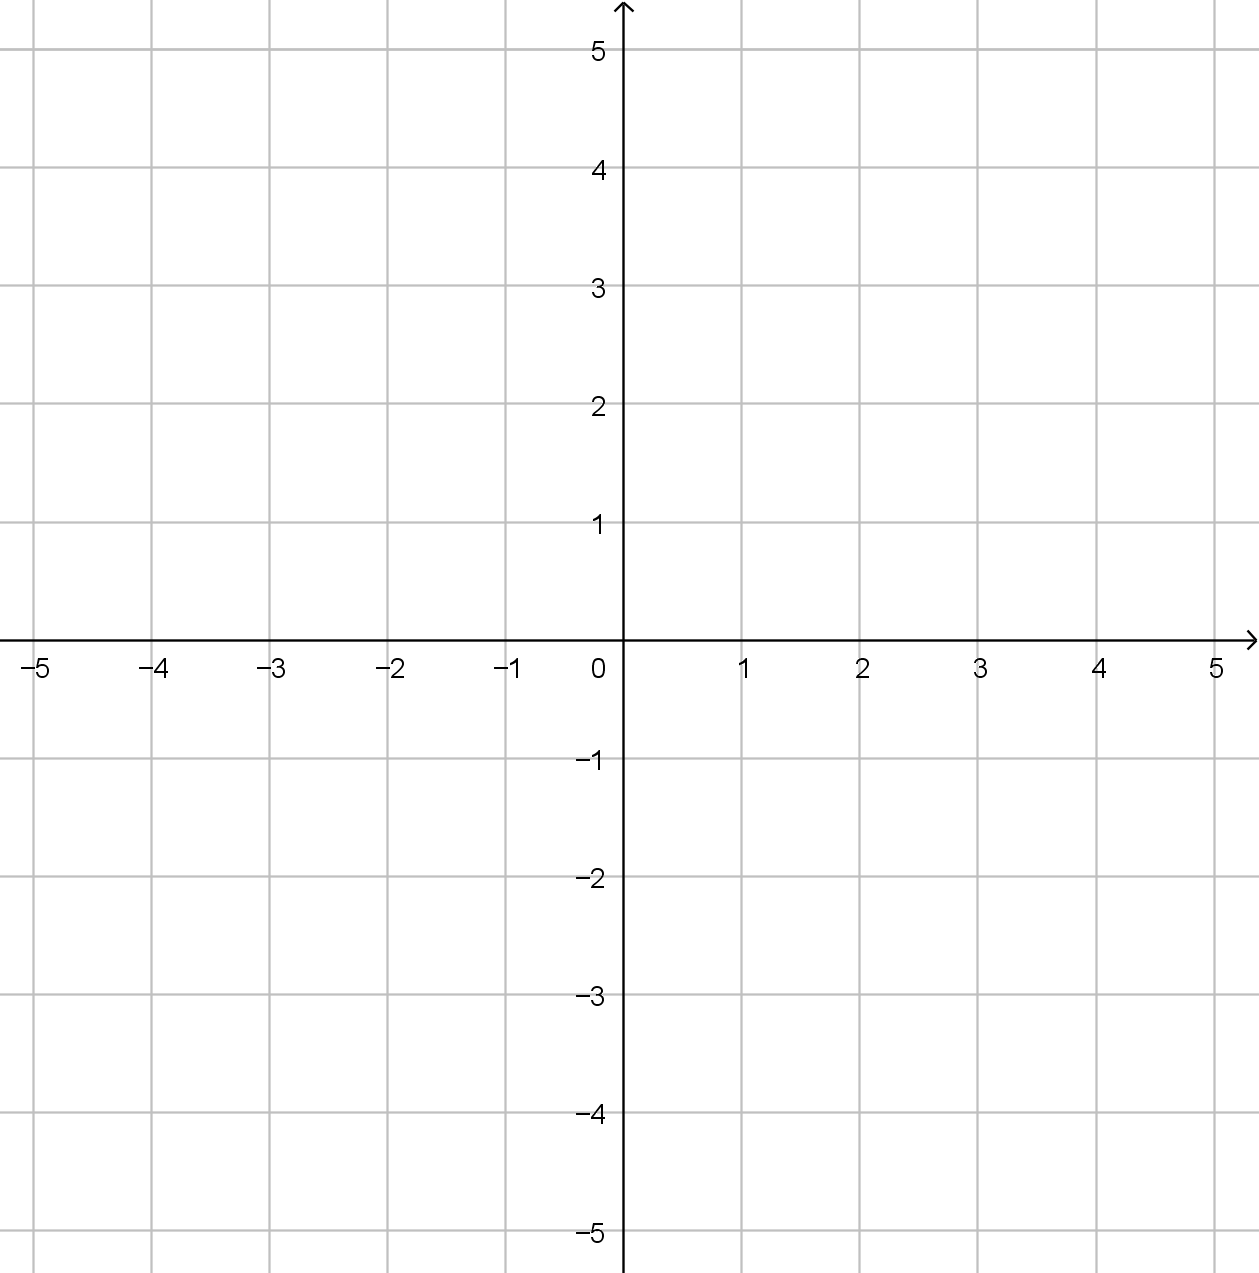
\includegraphics[width=0.6\textwidth]{55grid}
\end{center}


\newpage
\begin{mdframed}
%
\revi{함수, 일대일함수, 일대일대응, 역함수}
\begin{enumerate}\label{review3}
\item
두 집합 \(X\), \(Y\)에 대하여 집합 \(X\)의 모든 원소 \(x\)가 집합 \(Y\)의 한 원소 \(y\)에 대응되는 것을 함수라고 한다.%
\item
함수 \(f:X\to Y\)가
\[x_1\neq x_2\Longrightarrow f(x_1)\neq f(x_2)\]
이면 \(f\)를 일대일함수라고 부른다.
(단, \(x_1,x_2\in X\))
\item
함수 \(f\)가 일대일함수이고,  공역과 치역이 같으면 \(f\)를 일대일대응이라고 부른다.
\item
함수 \(f:X\to Y\)가 일대일대응일 때, \(f\)의 역함수 \(f^{-1}:Y\to X\)는
\[y=f(x)\iff x=f^{-1}(y)\]
를 만족시키는 함수이다.
\(f\)의 그래프와 \(f^{-1}\)의 그래프는 직선 \(y=x\)에 대하여 대칭이다.
\end{enumerate}
\end{mdframed}

%
\prob{}\label{review4}
다음  세 개의 대응 중 함수의 개수를 \(a\), 일대일함수의 개수를 \(b\),  일대일대응의 개수를 \(c\)라고 할 때, \(a\), \(b\), \(c\)의 값을 각각 구하여라.
\bigskip
\bigskip
\begin{center}
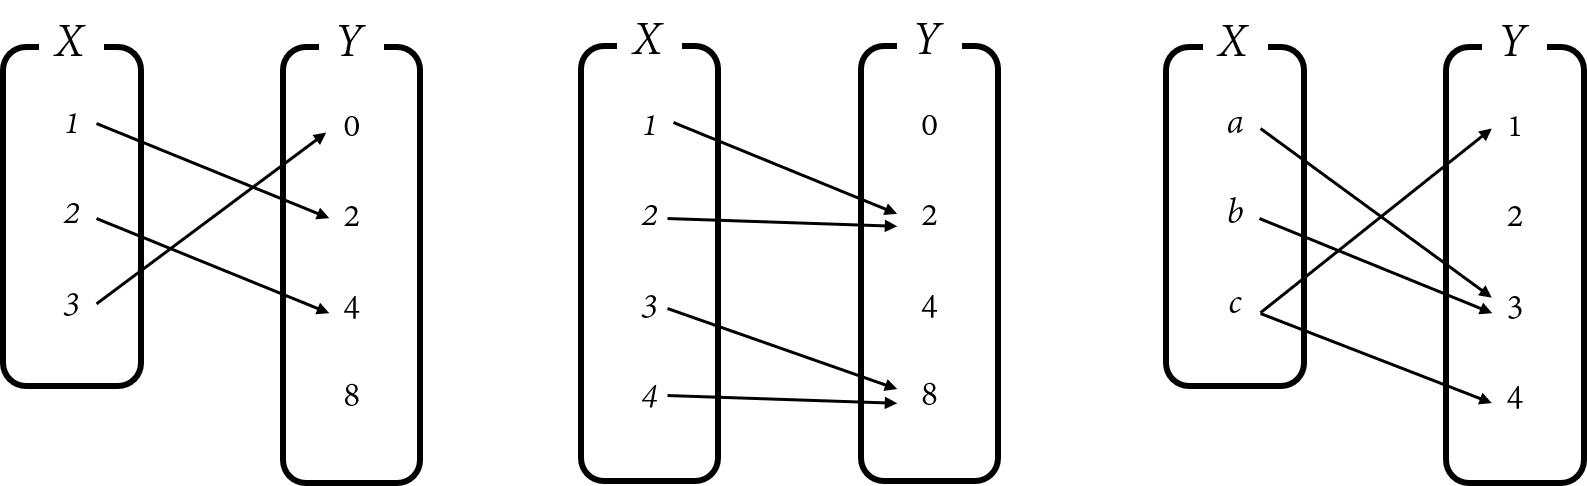
\includegraphics[width=0.7\textwidth]{review_4}
\end{center}

\newpage
\begin{mdframed}
%
\defi{증가함수, 감소함수}\label{review5}
함수 \(f:X\to Y\)가
\begin{enumerate}
\item
\(x_1<x_2\Longrightarrow f(x_1)<f(x_2)\)
이면 \(f\)를 증가함수라고 부른다.
\item
\(x_1<x_2\Longrightarrow f(x_1)>f(x_2)\)
이면 \(f\)를 감소함수라고 부른다.
\end{enumerate}
\end{mdframed}
따라서 증가함수와 감소함수는 일대일함수이다.

%
\exam{}
\begin{enumerate}\label{review6}
\item
\(f(x)=\sqrt x\)는, \(0\le x_1<x_2\)일 때 \(\sqrt{x_1}<\sqrt{x_2}\)이므로 \(f(x_1)<f(x_2)\)이다.
따라서 \(f\)는 증가함수이다.
\item
\(g(x)=-x+2\)는, \(x_1<x_2\)일 때 \(-x_1>-x_2\), \(-x_1+2>-x_2+2\)이므로 \(g(x_1)>g(x_2)\)이다.
따라서 \(f\)는 감소함수이다.
\end{enumerate}
\begin{center}
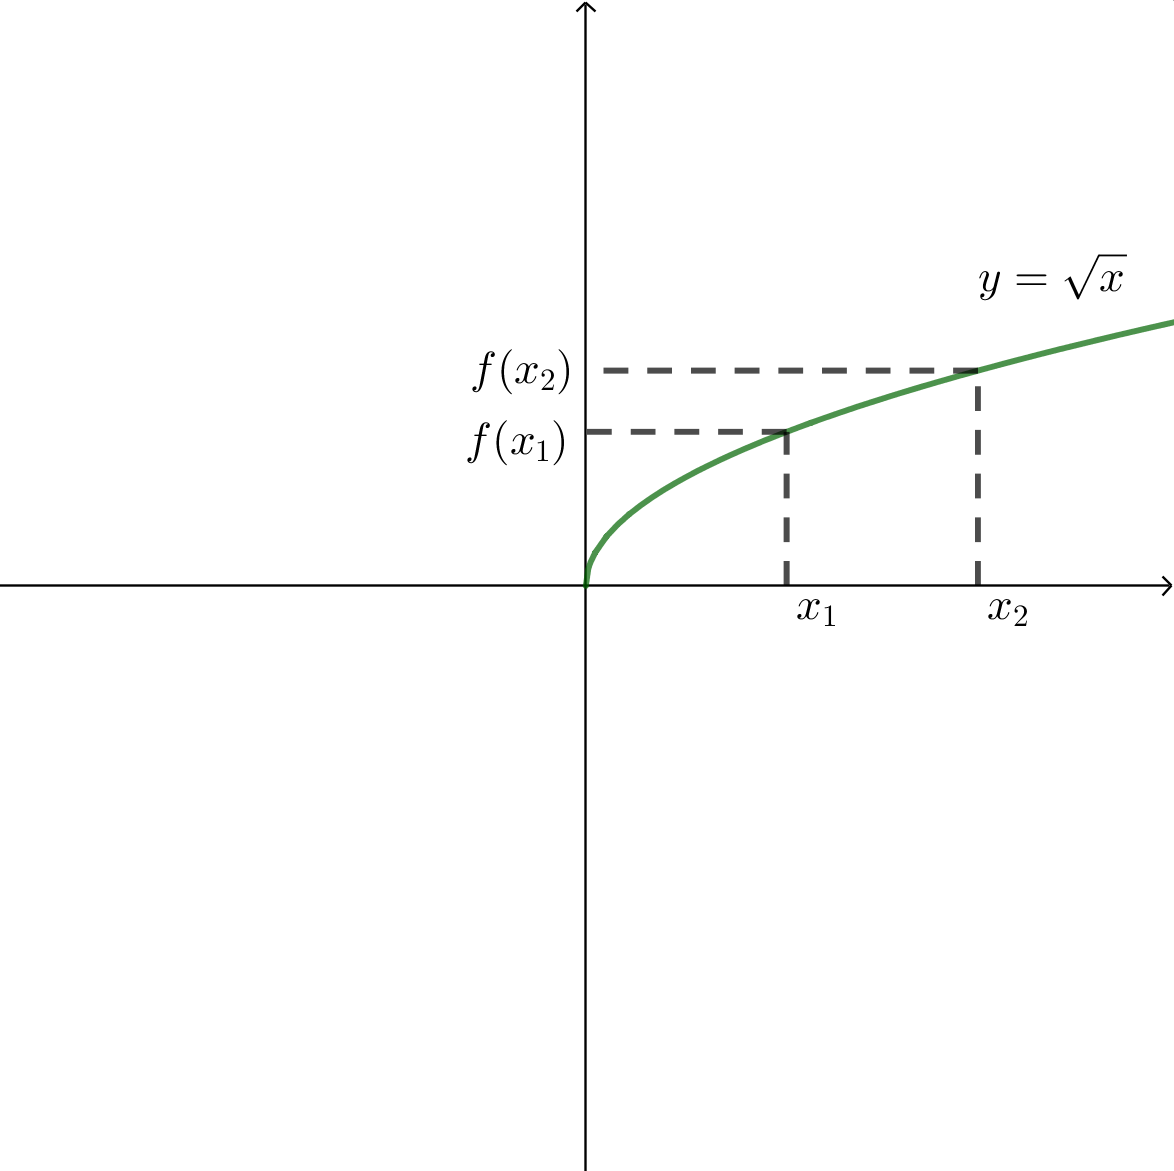
\includegraphics[width=0.45\textwidth]{review_6-1}
\quad
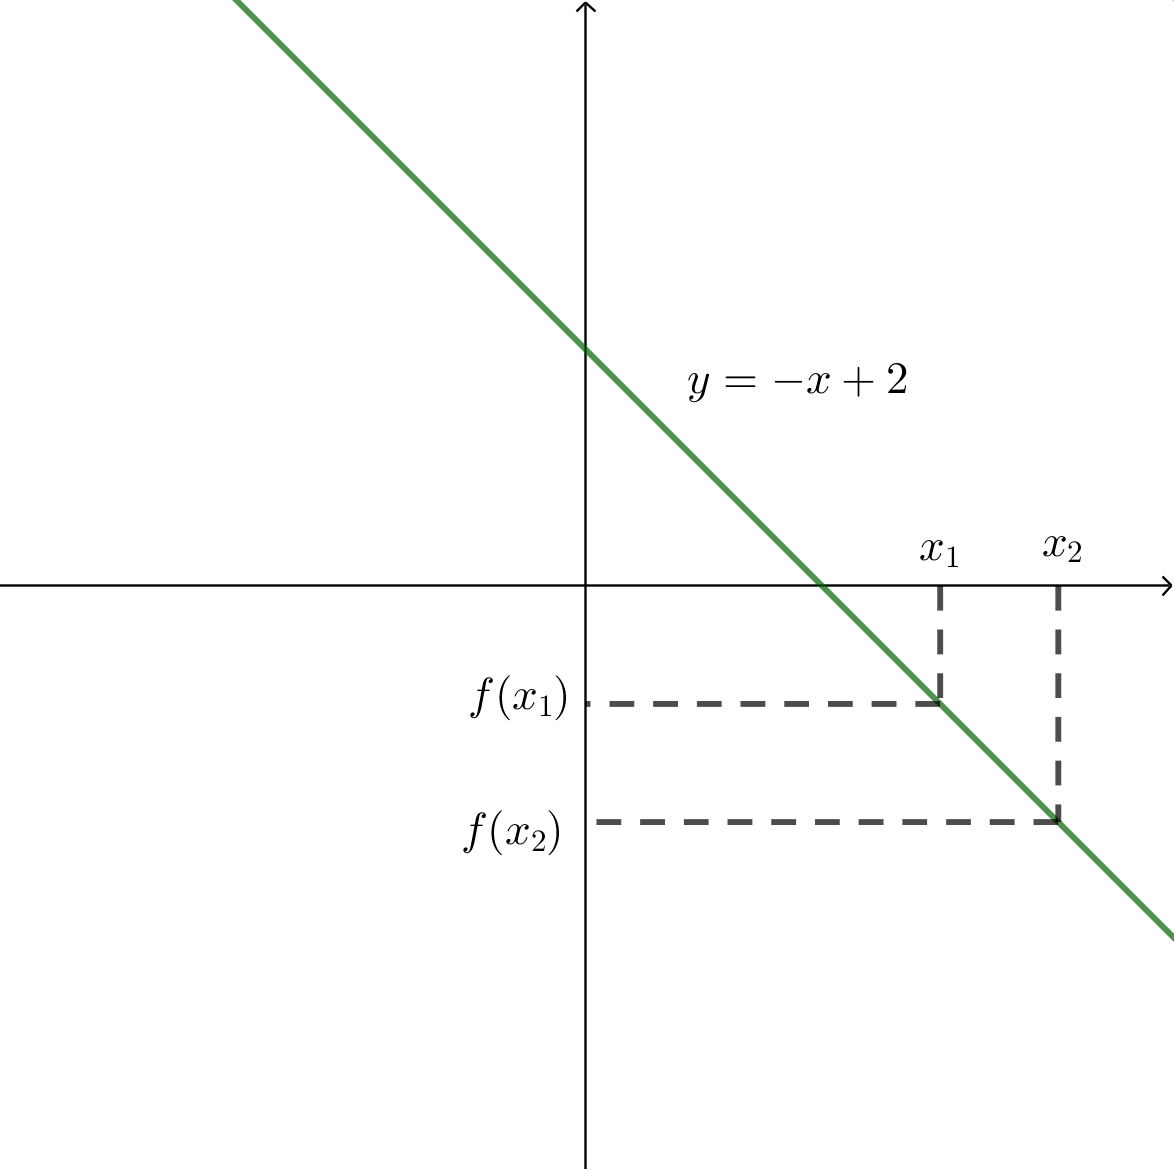
\includegraphics[width=0.45\textwidth]{review_6-2}
\end{center}

%
\prob{다음 빈칸에 알맞은 것을 써넣어라.}
\begin{enumerate}\label{review7}
\item
함수 \(y=\frac12x-1\)은 \pb{증가}함수이다.
\item
함수 \(y=-\sqrt{-x+3}+1\)는 \pb{증가}함수이다.
\item
함수 \(y=x^2\)은 \(x\le0\)에서 \pb{증가}함수이고 \(x\ge0\)에서는 \pb{감소}함수이다.
\end{enumerate}

\newpage
%
\prob{다음 빈칸에 알맞은 것을 써넣어라.}
\begin{enumerate}\label{review8}
\item
함수 \(f(x)=2x+4\)는 일대일대응이고 \(f\)의 역함수는 \(f^{-1}(x)=\pb{\frac12x-2}\)이다.
이때 \(f\)의 정의역은 실수 전체의 집합이고 \(f\)의 공역도 실수 전체의 집합이다.
\item
함수 \(g(x)=\frac1{x+2}+3\)는 일대일대응이고 \(g\)의 역함수는 \(g^{-1}(x)=\frac1{x-3}-2\)이다.
이때 \(g\)의 정의역은 \(\{x\ba x\neq-2\}\)이고 \(g\)의 공역은 \(\pb{\{y\ba y\neq3\}}\)이다.
\item
함수 \(h(x)=\sqrt{x-2}-1\)는 일대일대응이고 \(h\)의 역함수는\\ \(h^{-1}(x)=(x+1)^2+2(x\ge-1)\)이다.
이때 \(h\)의 정의역은 \(\pb{\{x\ba x\ge2\}}\)이고 \(h\)의 공역은 \(\{y\ba y\ge-1\}\)이다.
\end{enumerate}

%
\prob{두 집합 \(X=\{3,5,7\}\), \(Y=\{1,2,3,4,5\}\)에 대하여 다음을 구하여라.}
\begin{enumerate}\label{review9}
\item
함수 \(f:X\to Y\)의 개수
\item
일대일함수 \(f:X\to Y\)의 개수
\item
증가함수 \(f:X\to Y\)의 개수
\item
감소함수 \(f:X\to Y\)의 개수
\end{enumerate}

\begin{center}
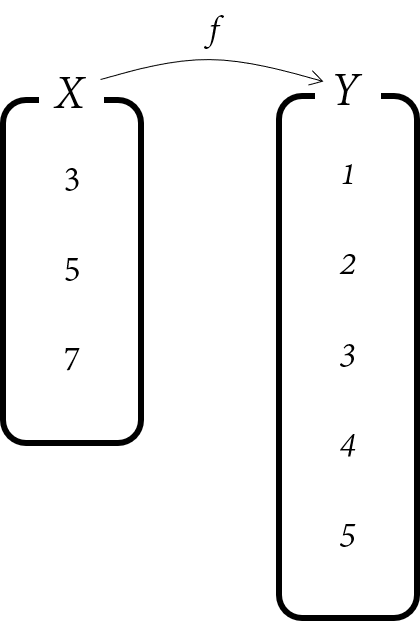
\includegraphics[width=0.3\textwidth]{review_9}
\end{center}

%%%
\section{지수함수의 그래프}

%
\exam{\(y=2^x\)의 그래프를 그려라.}\label{exp1}
\begin{mdframed}
\(y=2^x\)를 만족시키는 모든 점 \((x,y)\)를 표시하면 된다.
\(x=1\)이면 \(y=2\)이고 \(x=2\)이면 \(y=4\)이다.
따라서 \(y=2^x\)의 그래프는 \((1,2)\), \((2,4)\)와 같은 점들을 포함한다.
이밖에도
\begin{align*}
(x,y)
=&\textstyle(1,2),\:(2,4),\:(3,8),\:(4,16),\:\cdots\\
&\textstyle(0,1),\:(-1,\frac12),\:(-2,\frac14),\:(-3,\frac18)\:\cdots
\end{align*}
와 같은 점들을 찍을 수 있다.
이 점들을 자연스럽게 이으면 다음과 같은 곡선이 나온다.
\begin{center}
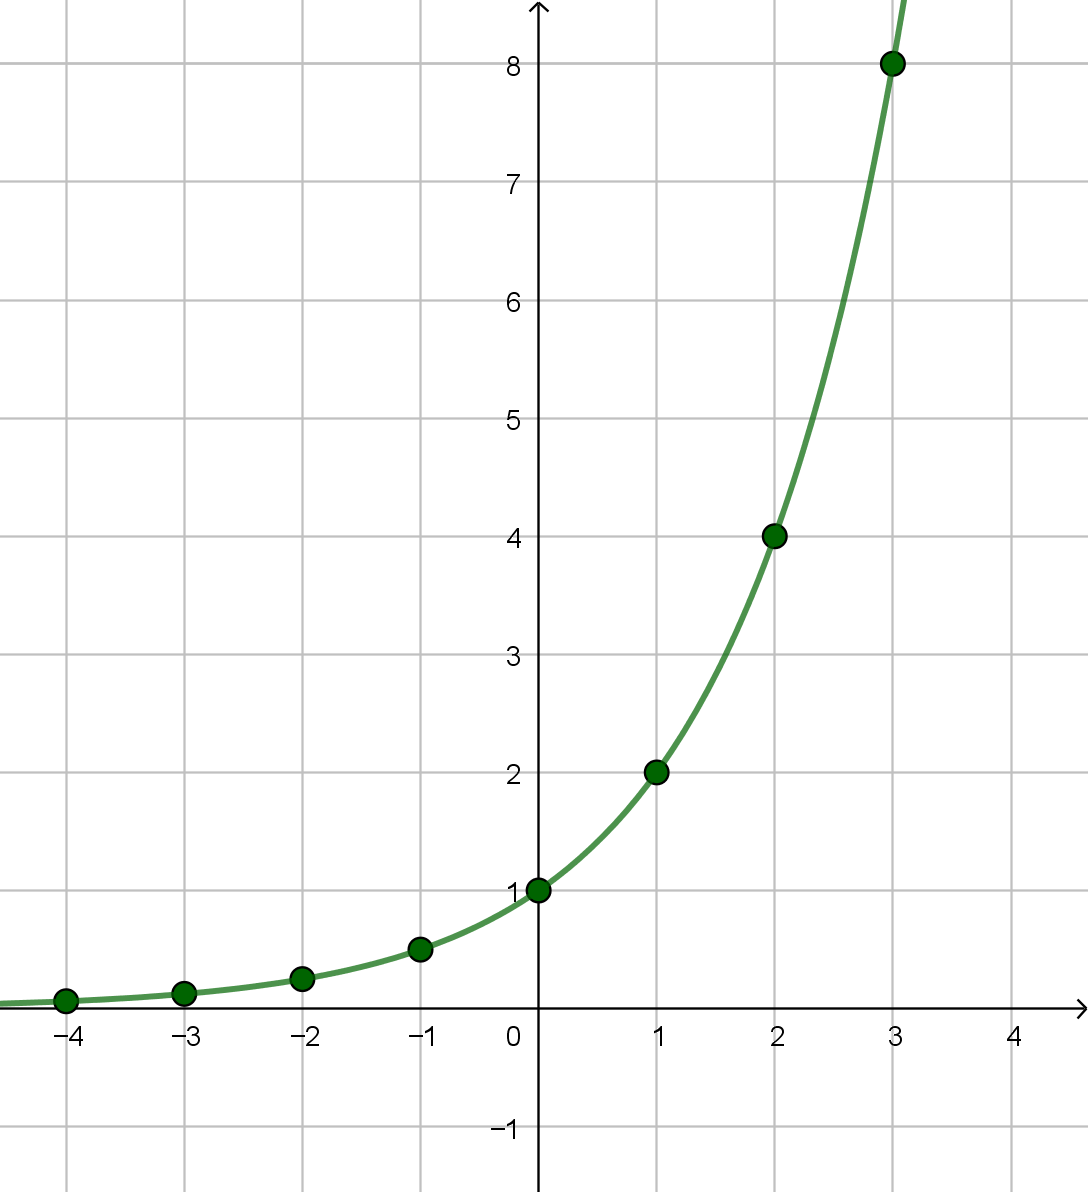
\includegraphics[width=0.6\textwidth]{exp_1}
\end{center}
\end{mdframed}

\newpage
%
\prob{다음 지수함수들의 그래프를 그려라.}
\begin{enumerate}\label{exp2}
\item
\(y=3^x\)
\item
\(y=(\frac12)^x\)
\item
\(y=(\frac13)^x\)
\end{enumerate}
\begin{center}
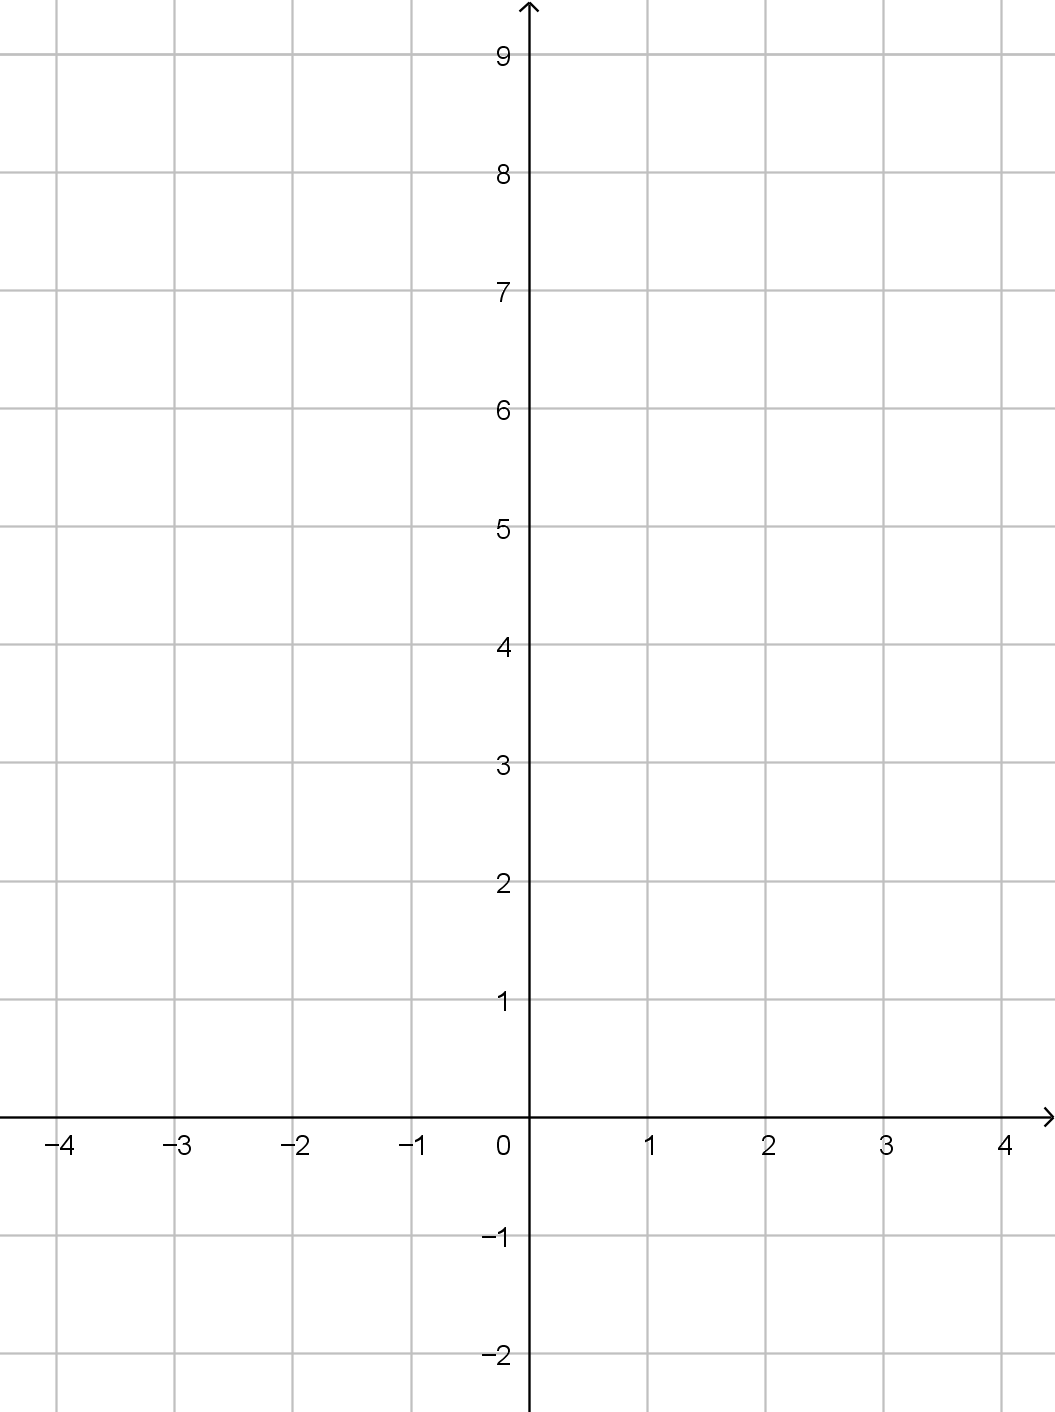
\includegraphics[width=0.6\textwidth]{49grid}
\end{center}

\begin{mdframed}
%
\theo{지수함수 \(y=a^x\)(\(a>0\), \(a\neq1\))의 성질}
\begin{itemize}\label{exp3}
\item
정의역은 실수 전체의 집합이고 치역은 양의 실수 전체의 집합이다.
\item
\(a>1\)이면 증가함수이고 \(0<a<1\)이면 감소함수이다.
\item
그래프는 \((0,1)\)을 지나고, \(x\)축을 점근선으로 갖는다.
\end{itemize}
\end{mdframed}

\newpage
%
\exam{함수 \(y=2^{x-1}-2\)의 그래프를 그리고, 점근선의 방정식을 구하시오.}\label{exp4}
\begin{mdframed}
함수 \(y=2^x\)의 그래프를 \(x\)축의 방향으로 1만큼 \(y\)축의 방향으로 \(-2\)만큼 평행이동하면 된다.
따라서 다음과 같은 그래프가 나온다.
\begin{center}
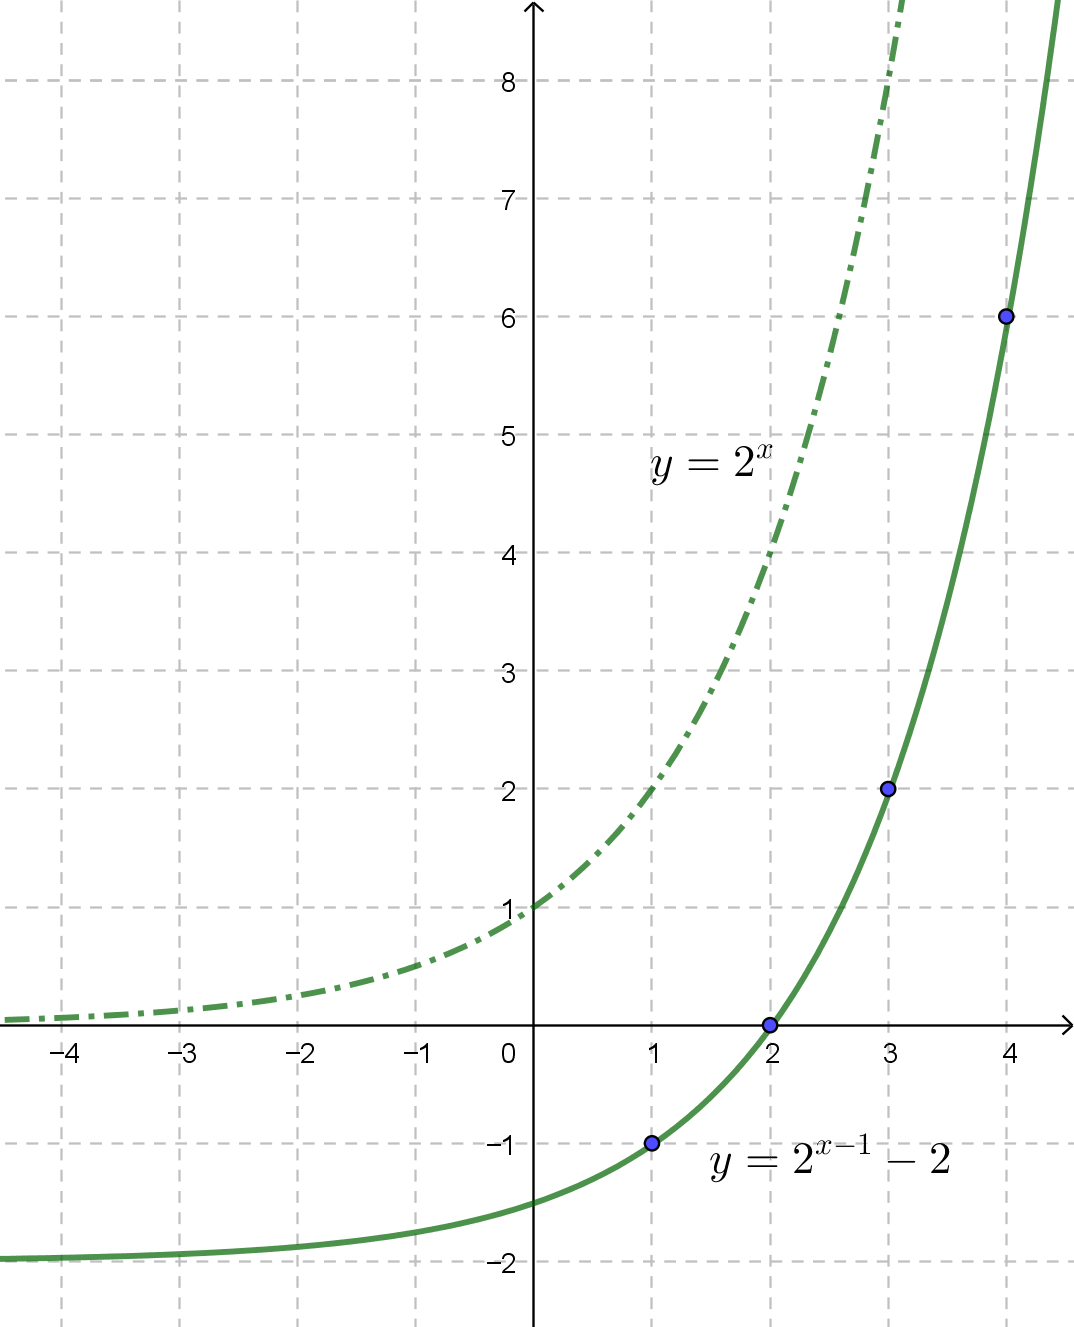
\includegraphics[width=0.6\textwidth]{exp_4}
\end{center}
이때 점근선의 방정식은 \(y=-2\)이다.
\end{mdframed}

\newpage
%
\prob{다음 지수함수들의 그래프를 그리고, 점근선의 방정식을 구하시오.}\label{exp5}
\begin{enumerate}
\item
\(y=3^{x+1}-2\)
\item
\(y=-(\frac13)^{-x}\)
\end{enumerate}

\begin{center}
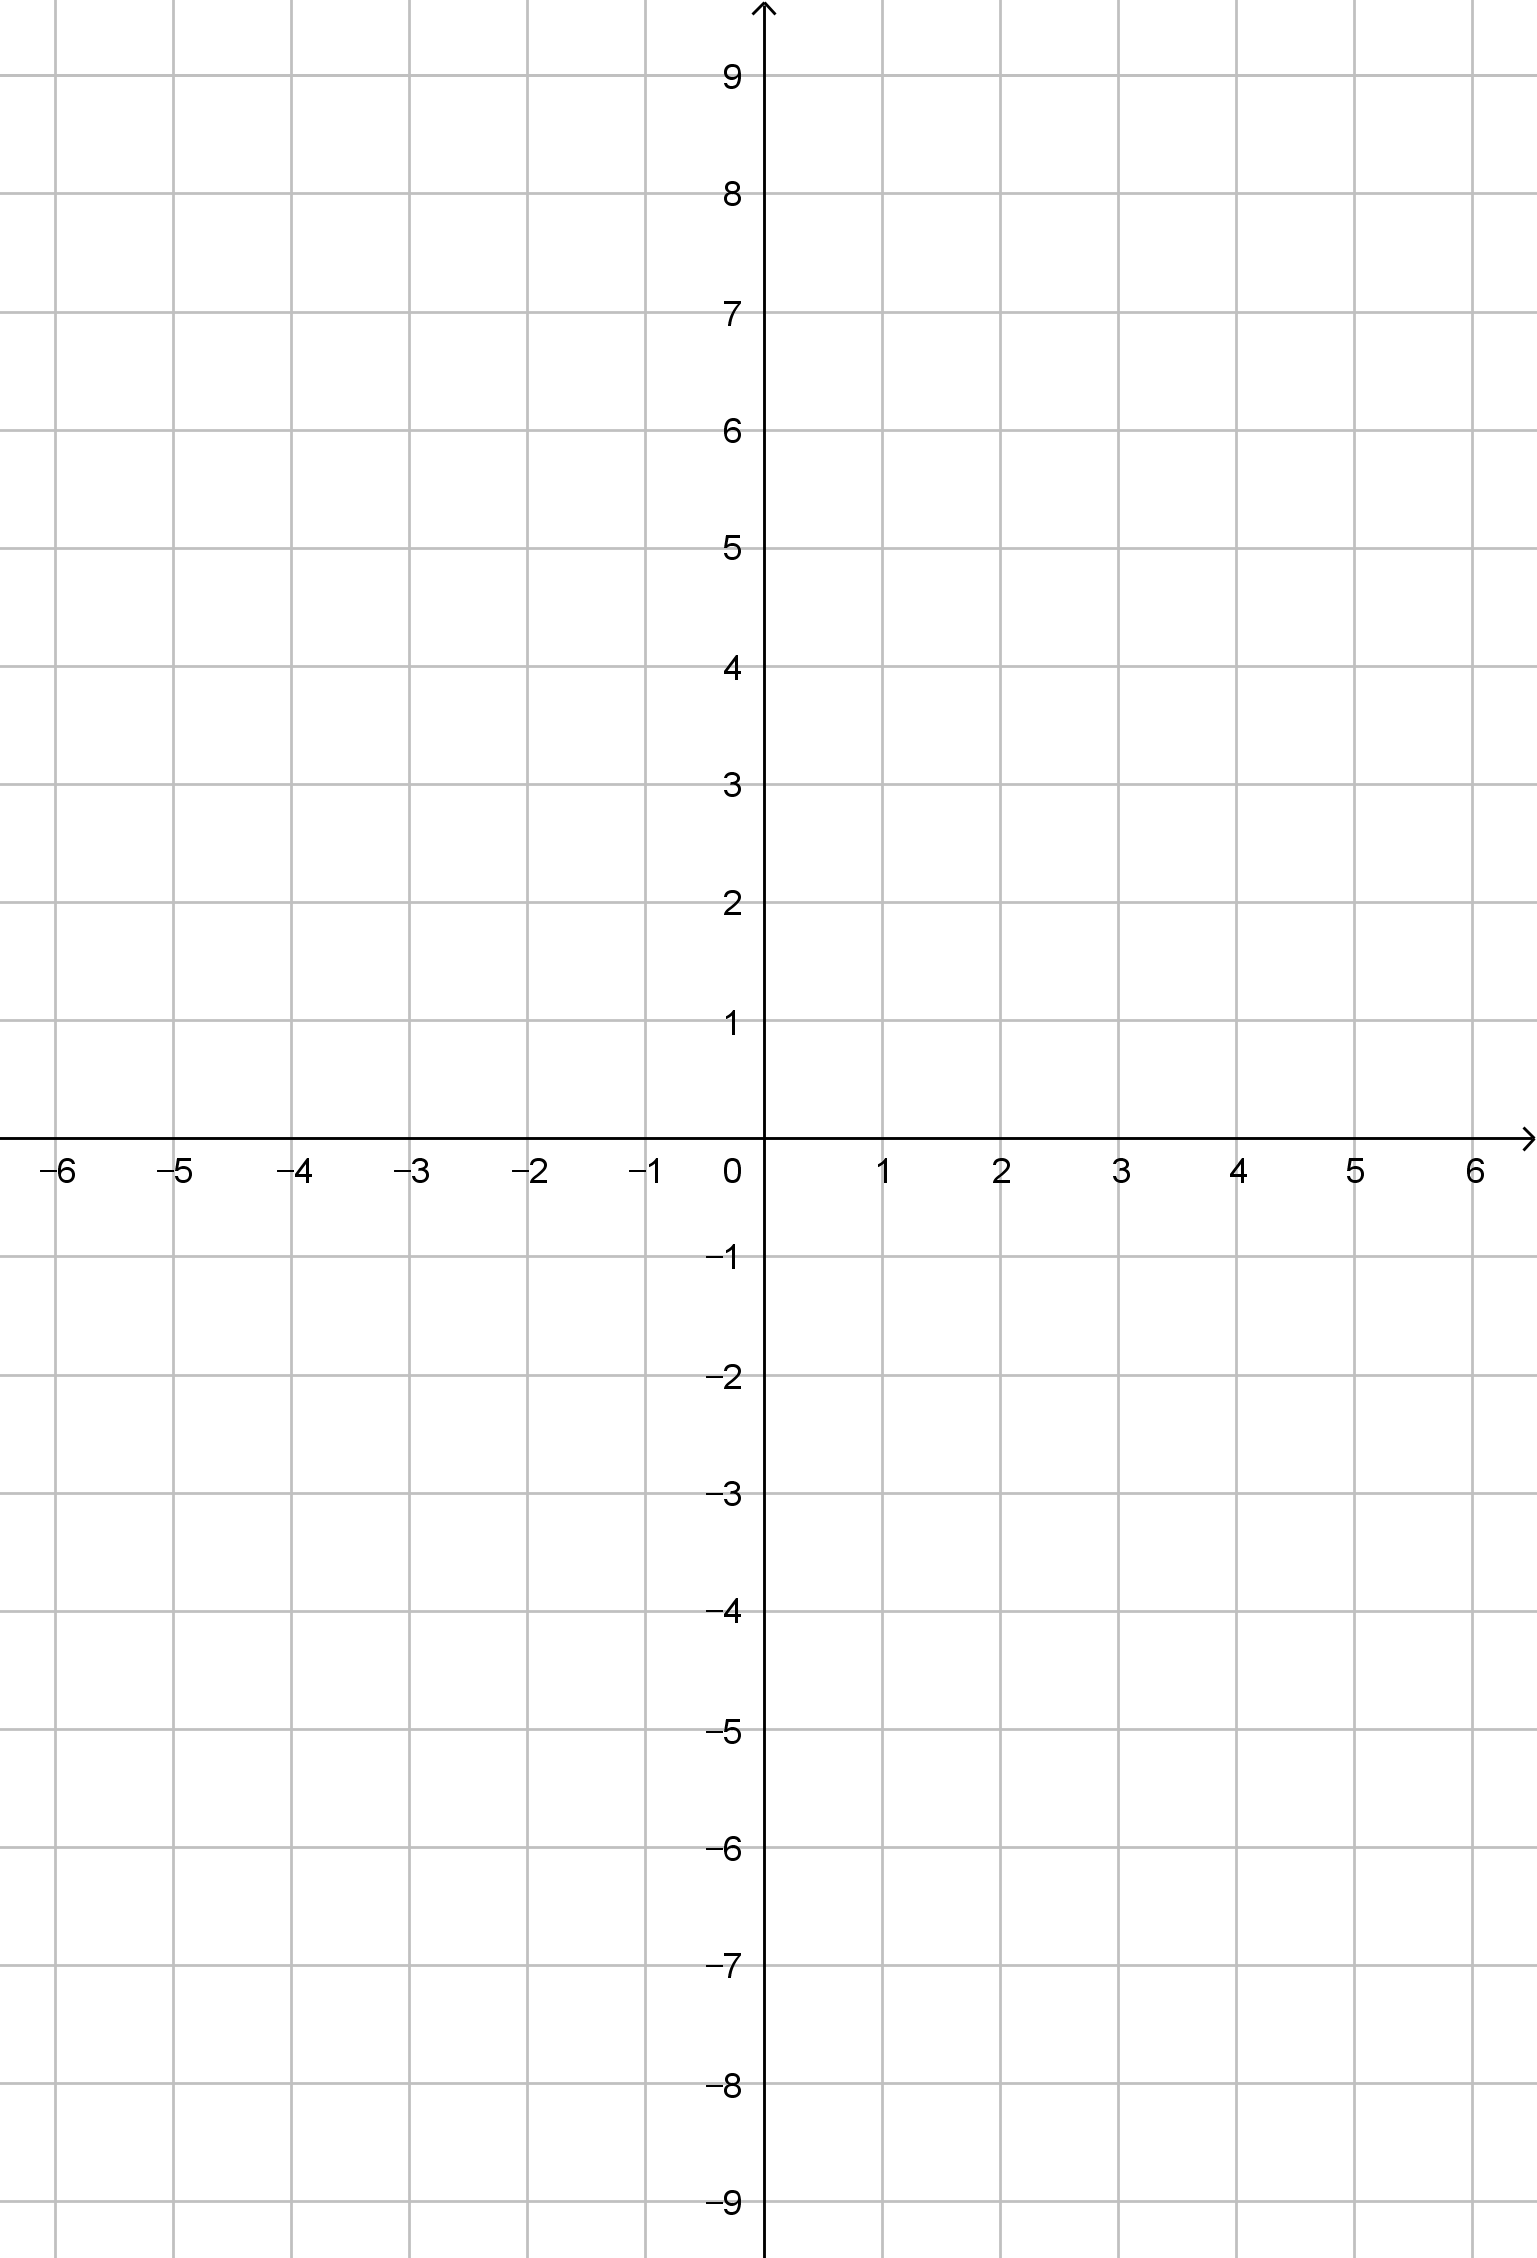
\includegraphics[width=0.8\textwidth]{69grid}
\end{center}

%%%
\section{로그함수의 그래프}

%
\exam{\(y=\log_2x\)의 그래프를 그려라.}\label{log1}
\begin{mdframed}
\(y=\log_2x\)를 만족시키는 모든 점 \((x,y)\)를 표시하면 된다.
이때 \(x\)는 진수이므로 \(x\)에는 양수만 대입할 수 있다.
\(x=2\)이면 \(y=1\)이고 \(x=4\)이면 \(y=2\)이다.
따라서 \(y=2^x\)의 그래프는 \((2,1)\), \((4,2)\)와 같은 점들을 포함한다.
이밖에도
\begin{align*}
(x,y)
=&\textstyle(2,1),\:(4,2),\:(8,3),\:(16,4),\:\cdots\\
&\textstyle(1,0),\:(\frac12,-1),\:(\frac14,-2),\:(\frac18,-3)\:\cdots
\end{align*}
와 같은 점들을 찍을 수 있다.
이 점들을 자연스럽게 이으면 다음과 같은 곡선이 나온다.
\begin{center}
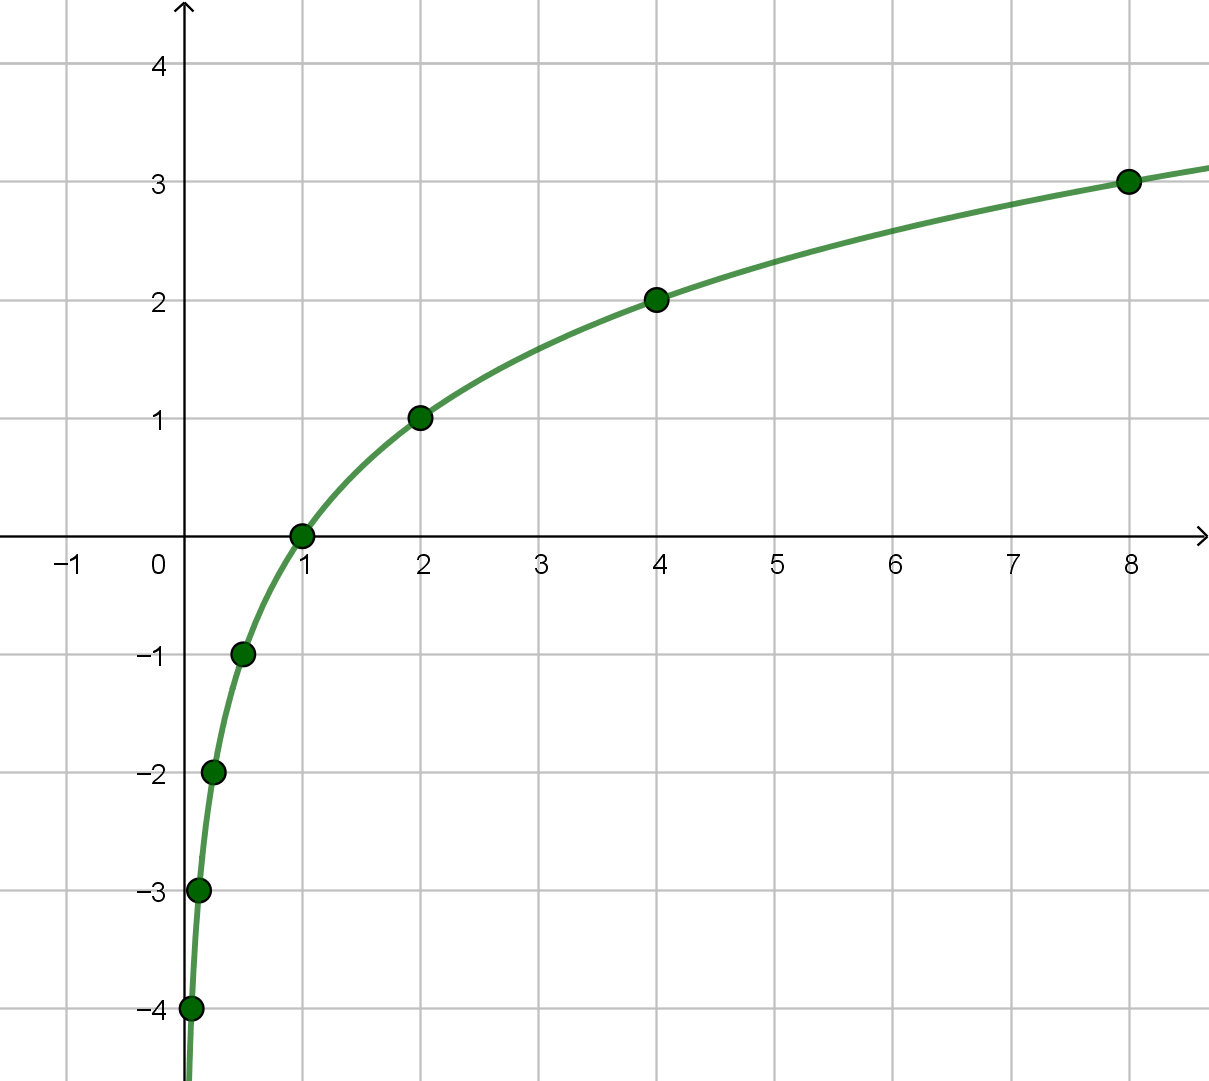
\includegraphics[width=0.6\textwidth]{log_1}
\end{center}
\end{mdframed}

\bigskip\bigskip
함수 \(y=\log_2x\)는 지수함수 \(y=2^x\)의 역함수이기도 하다.
따라서 \(y=2^x\)의 그래프를 직선 \(y=x\)에 대하여 대칭이동시켜서 얻을 수도 있다.

\newpage
%
\prob{다음은 지수함수 \(y=2^x\)의 역함수를 구하는 과정이다. \fbox{(A)}에 알맞은 집합을 고르시오.}\label{log2}\\[-30pt]
\begin{mdframed}[innertopmargin=5pt]
함수 \(f(x)=2^x\)의 정의역은 실수 전체의 집합이고 치역은 \fbox{(A)}이다.
따라서 \(f\)의 공역을 \fbox{(A)}로 잡으면 \(f\)는 일대일대응이 되고, 역함수가 존재한다.
\(f\)의 역함수를 구하기 위해
\[x=2^y\]
로 놓으면
\[y=\log_2x\]
가 된다.
즉 \(f^{-1}(x)=\log_2x\)이다.
이때 \(f^{-1}\)의 정의역은 \fbox{(A)}이고 공역은 실수 전체의 집합이다.
\end{mdframed}
\tabb
{실수 전체의 집합}
{\(\{y\ba y<0\}\)}
{\(\{y\ba y\le0\}\)}
{\(\{y\ba y>0\}\)}
{\(\{y\ba y\ge0\}\)}

%
\prob{다음 로그함수들의 그래프를 그려라.}\label{log3}
\begin{enumerate*}[itemjoin=\qquad\qquad]
\item
\(y=\log_3x\)
\item
\(y=\log_{\frac12}x\)
\item
\(y=\log_{\frac13}x\)
\end{enumerate*}
\begin{center}
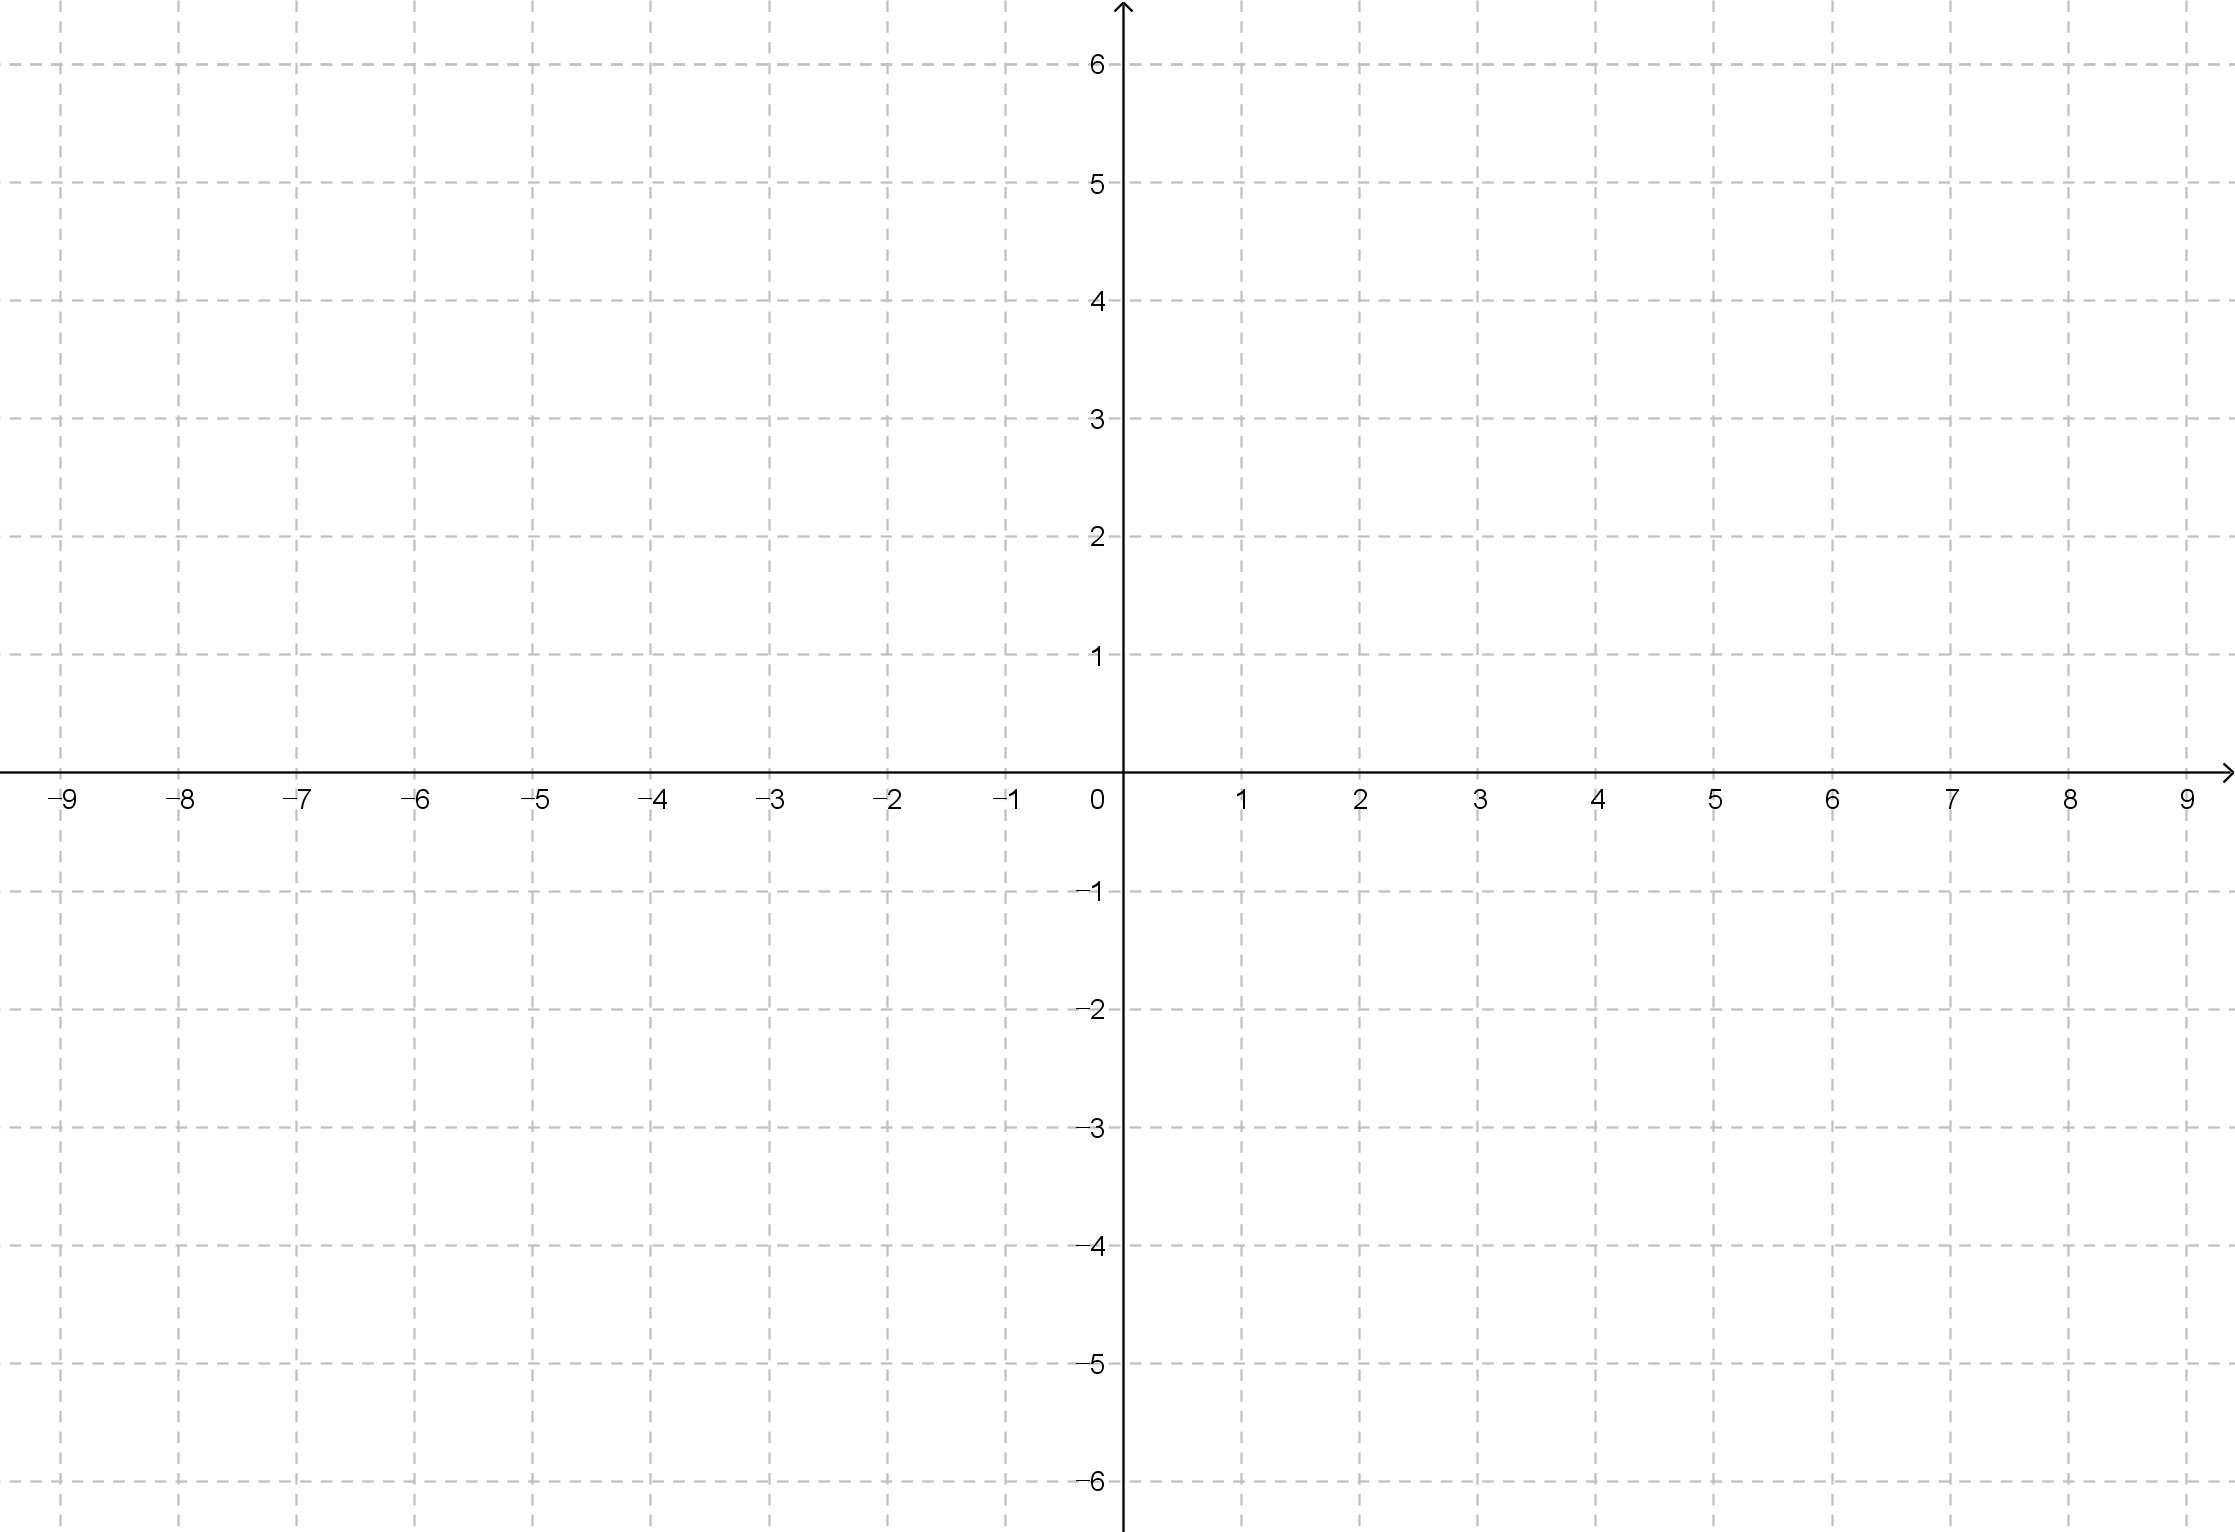
\includegraphics[width=\textwidth]{96grid}
\end{center}

\newpage
\begin{mdframed}
%
\theo{로그함수 \(y=\log_ax\)(\(a>0\), \(a\neq1\))의 성질}
\begin{itemize}\label{log4}
\item
정의역은 양의 실수 전체의 집합이고 치역은 실수 전체의 집합이다.
\item
\(a>1\)이면 증가함수이고 \(0<a<1\)이면 감소함수이다.
\item
그래프는 \((1,0)\)을 지나고, \(y\)축을 점근선으로 갖는다.
\end{itemize}
\end{mdframed}

%
\exam{함수 \(y=\log_2(-x+1)+2\)의 그래프를 그리고, 점근선의 방정식을 구하시오.}\label{log5}\\[-30pt]
\begin{mdframed}
함수 \(y=\log_2x\)의 그래프를 \(y\)축을 기준으로 대칭시켜 \(y=\log_2(-x)\)의 그래프를 얻고, 이것을 다시 \(x\)축의 방향으로 1만큼 \(y\)축의 방향으로 \(2\)만큼 평행이동하면 된다.
\[
y=\log_2x
\xrightarrow[대칭이동]{y축}
y=\log_2(-x)
\xrightarrow[평행이동]{\fbox{$x$}\::\:1,\quad\fbox{$y$}\::\:2}\
y=\log_2(-x+1)+2
\]
따라서 다음과 같은 그래프가 나온다.
\begin{center}
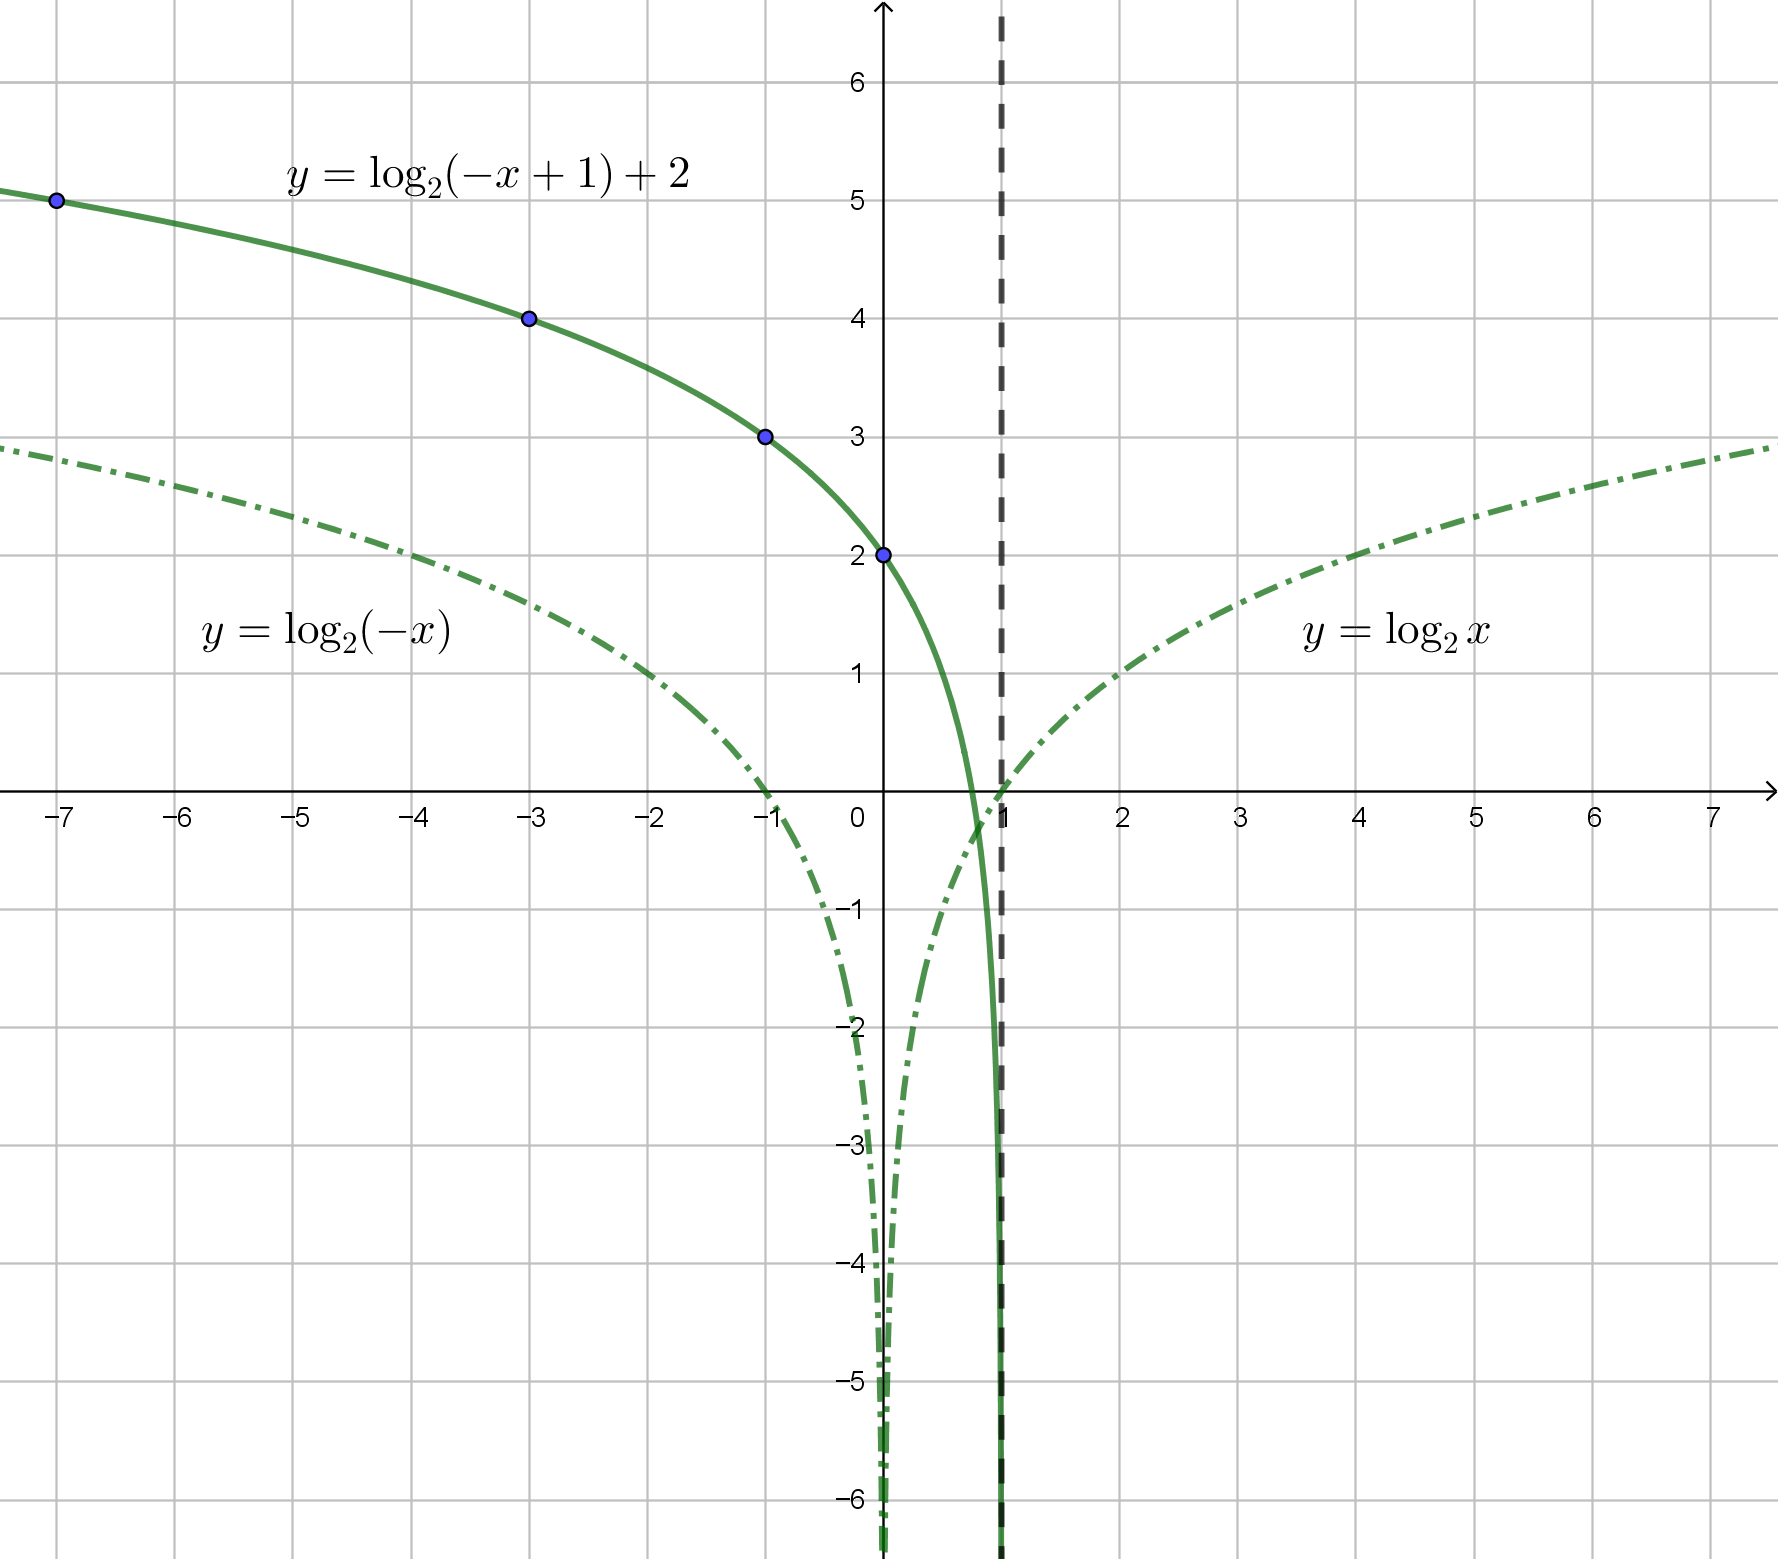
\includegraphics[width=0.6\textwidth]{log_5}
\end{center}
이때 점근선의 방정식은 \(x=1\)이다.
\end{mdframed}

\newpage
%
\prob{다음 로그함수들의 그래프를 그리고, 점근선의 방정식을 구하시오.}\label{log6}
\par\noindent
(1)\;\(y=\log_3(x+1)-1\)
\begin{center}
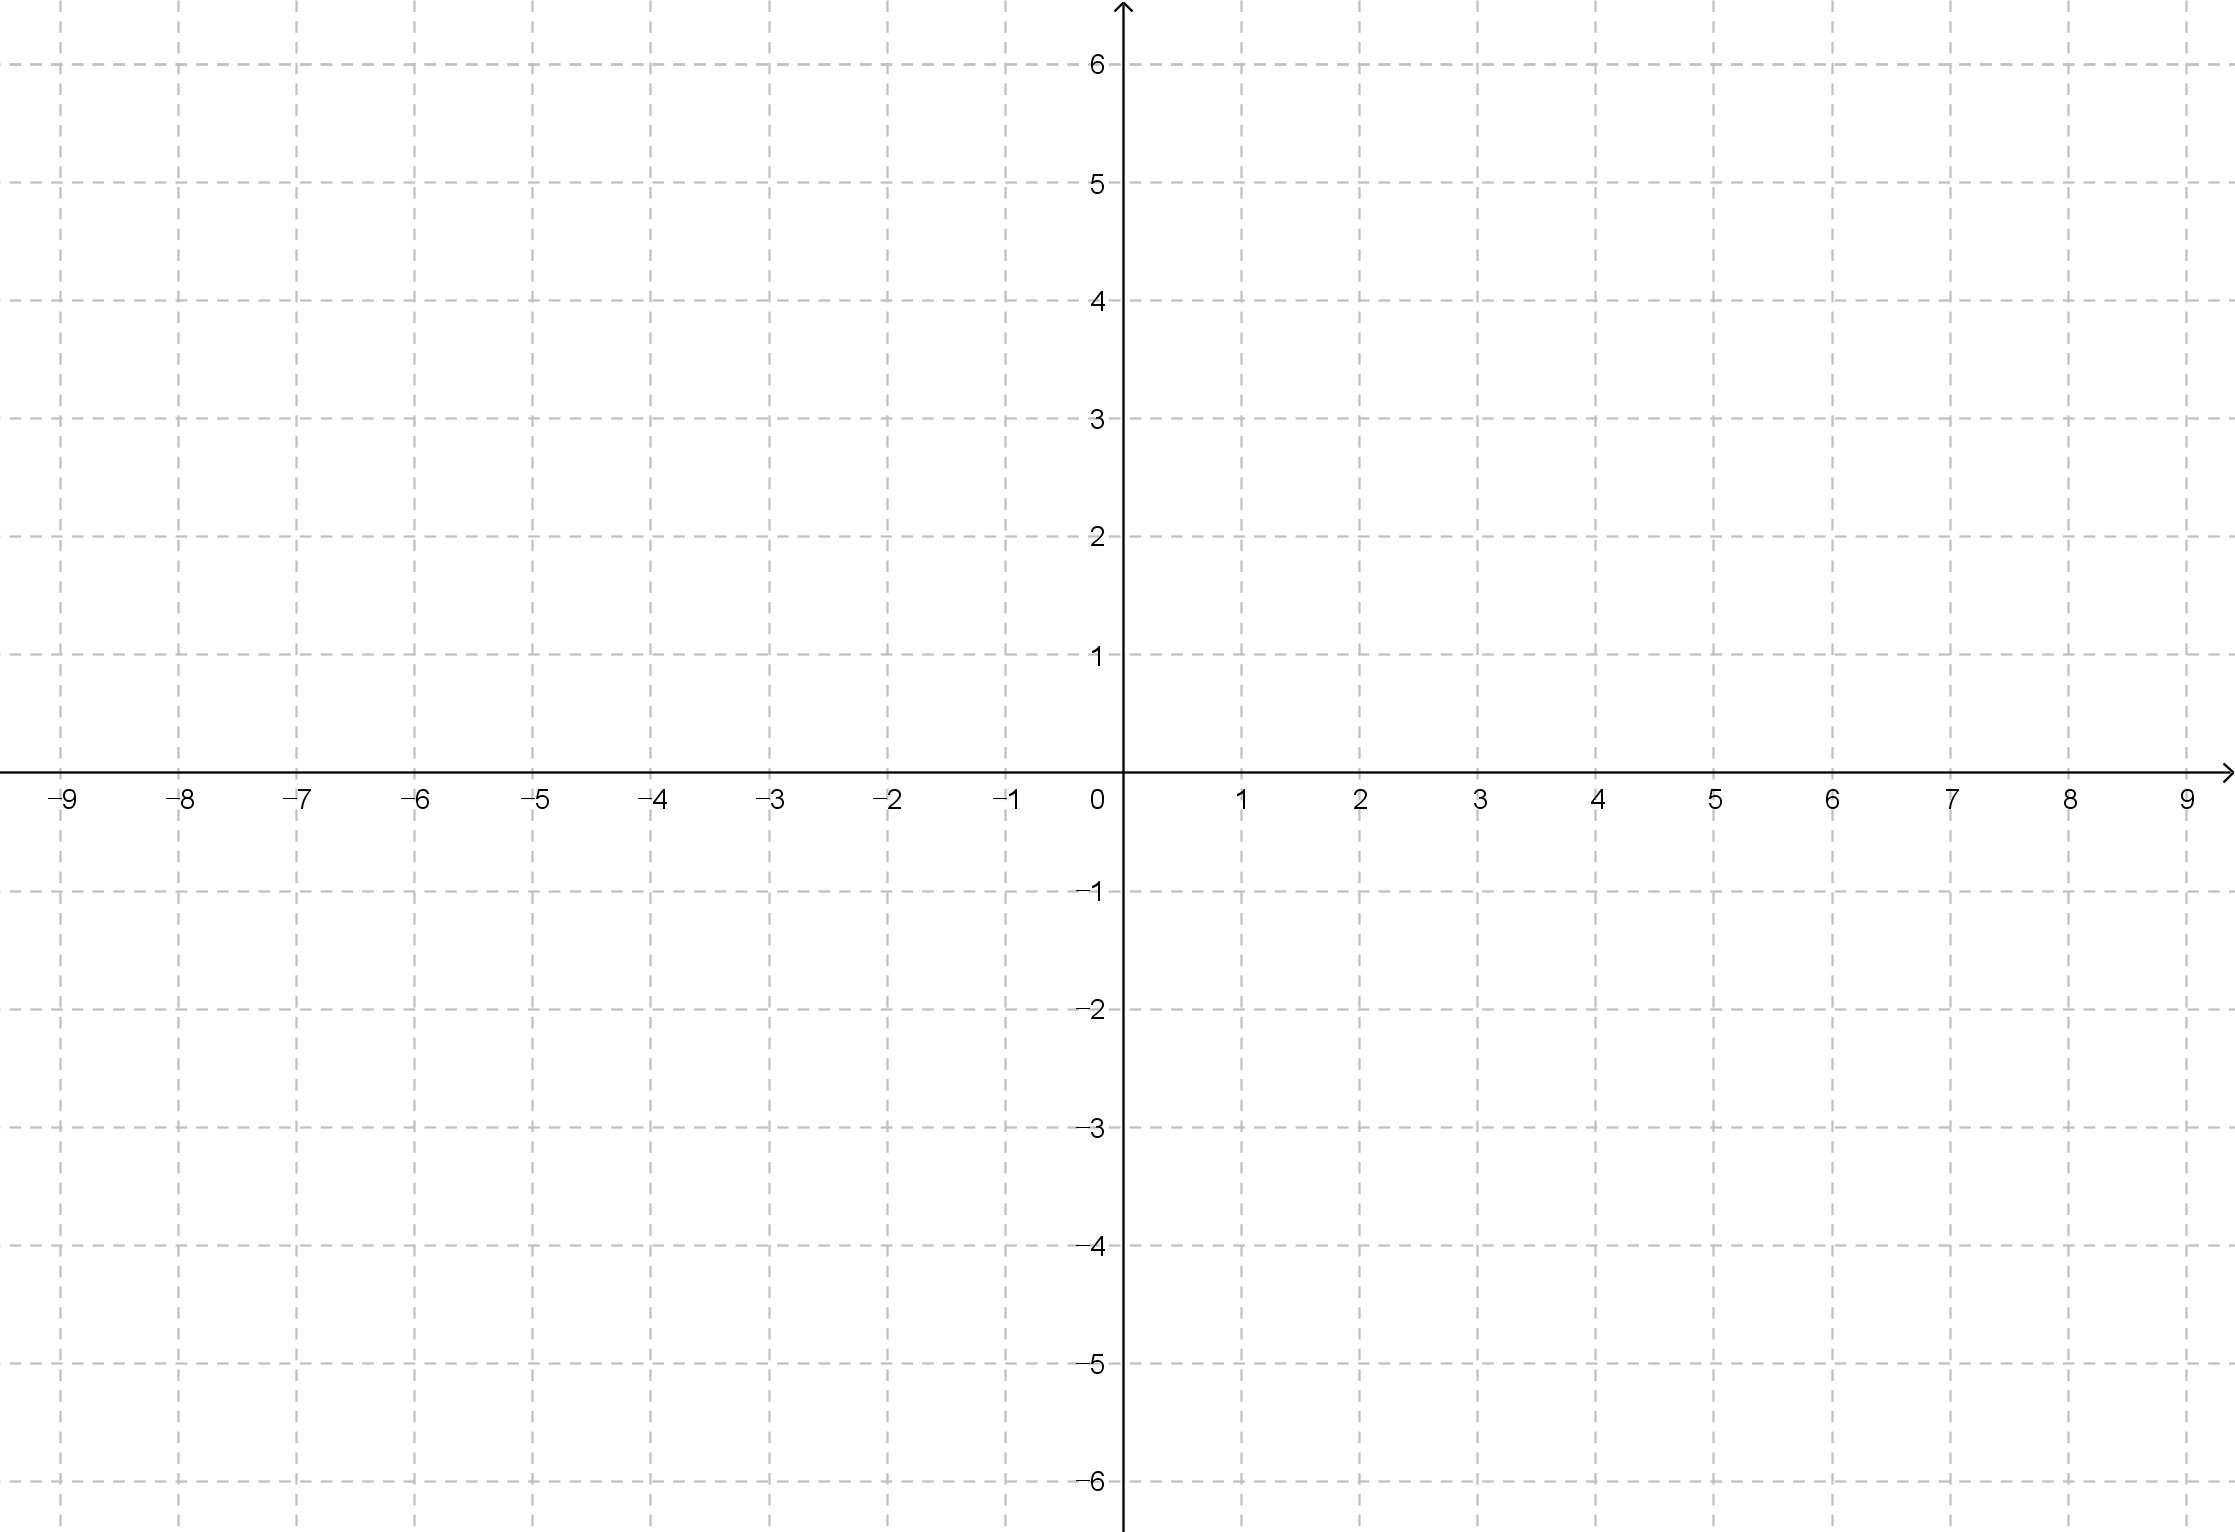
\includegraphics[width=\textwidth]{96grid}
\end{center}
\par\noindent
(2)\;\;\(y=-\log_3(-x)\)
\begin{center}
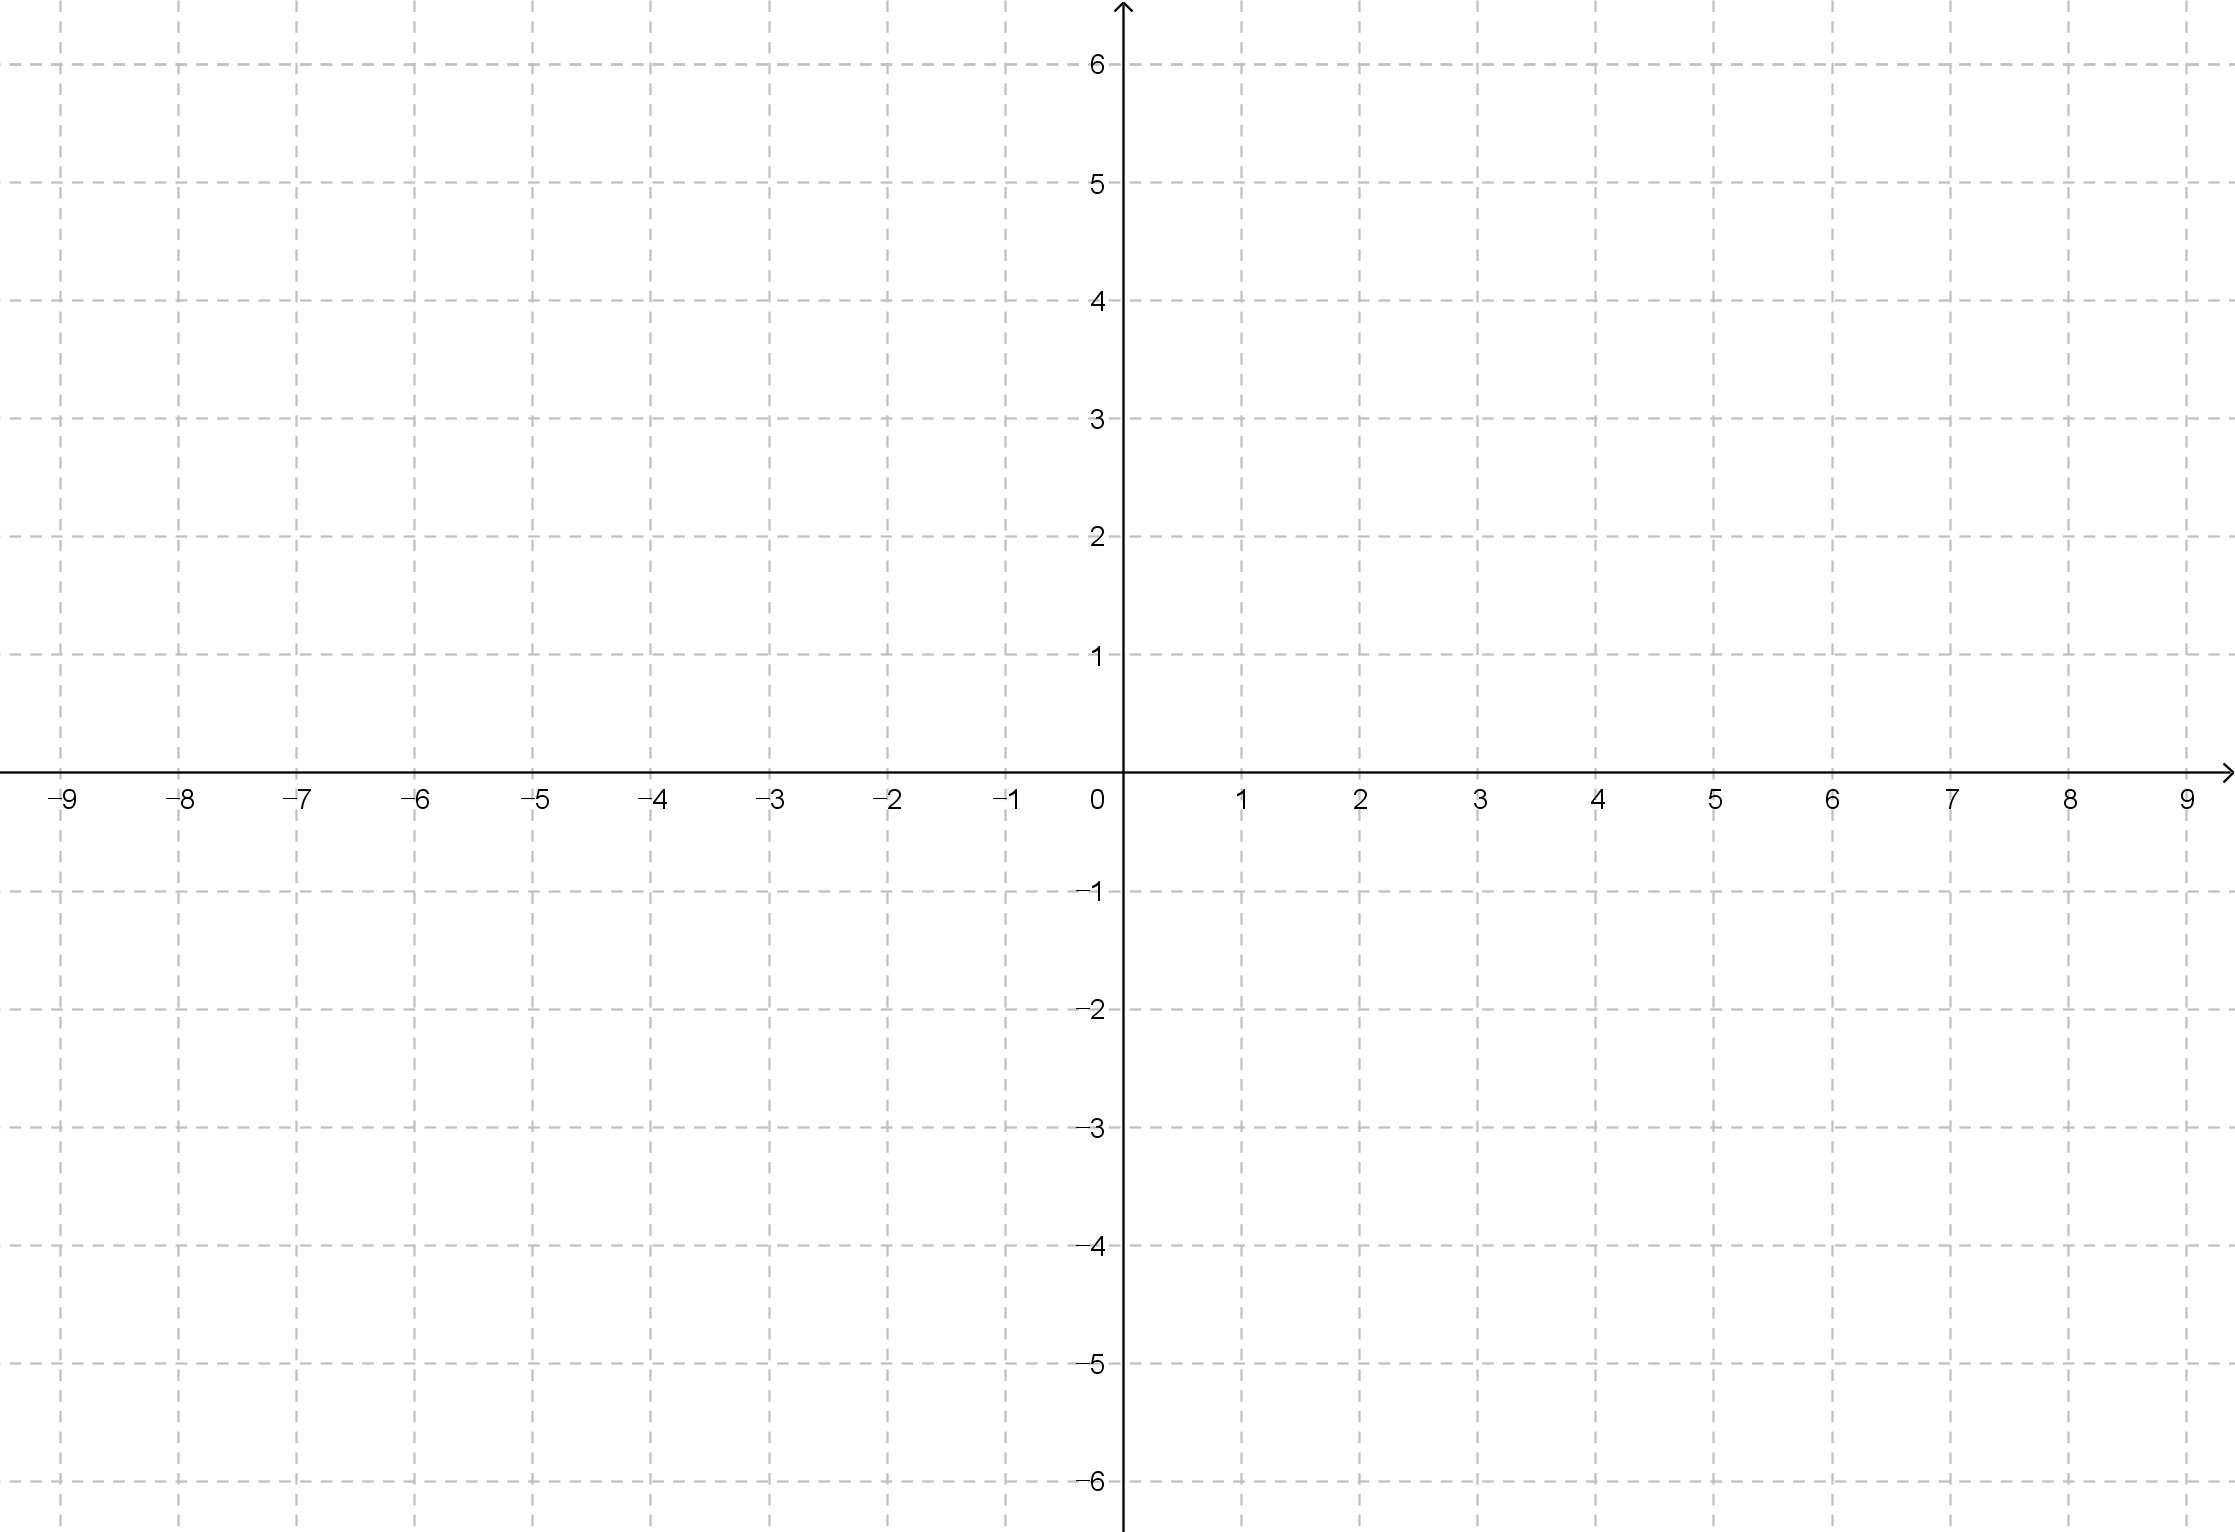
\includegraphics[width=\textwidth]{96grid}
\end{center}


%%%
\section{지수방정식과 로그방정식}
\(f:X\to Y\)가 함수이면 한 개의 \(x\)가 두 개 이상의 \(y\)에 대응되지 않는다.
따라서
\[x_1=x_2\quad\Longrightarrow\quad f(x_1)=f(x_2)\]
이다.
\(f\)가 일대일함수이면 두 개 이상의 \(x\)가 한 개의 \(y\)에 대응되지 않는다.
즉 \(x_1\neq x_2\)이면 \(f(x_1)\neq f(x_2)\)이다.
이것의 대우를 쓰면
\[f(x_1)=f(x_2)\quad\Longrightarrow\quad x_1=x_2\]
이다.
즉
\[x_1=x_2\quad\Longleftrightarrow\quad f(x_1)=f(x_2)\]
이다.
\(a>0\), \(a\neq1\)일 때, 지수함수 \(f(x)=a^x\)는 일대일함수이므로
\begin{mdframed}[innertopmargin=0pt,leftmargin=.23\textwidth,rightmargin=.23\textwidth]
\[x_1=x_2\quad\Longleftrightarrow\quad a^{x_1}=a^{x_2}\]
\end{mdframed}
이다.

%
\exam{\(2^{5x-2}=4^{x^2}\)을 만족시키는 \(x\)의 값을 구하여라.}\label{equa1}
\begin{mdframed}
\(2^{5x-2}=2^{2x^2}\)이므로 \(5x-2=2x^2\)이다.
\(2x^2-5x+2=0\), \((2x-1)(x-2)=0\)으로부터 \(x=\frac12,\;2\)이다.
\end{mdframed}
\ans{\(x=\frac12\) 또는 \(x=2\)}

%
\prob{다음 지수방정식을 푸시오.}\label{equa2}
\begin{enumerate*}[itemjoin=\tabto{.5\textwidth}]
\item
\(3^x-\sqrt3=0\)
\item
\(4^x=\frac1{32}\)
\end{enumerate*}

\newpage
로그함수 \(f(x)=\log_ax\) 또한 일대일함수이므로
\begin{mdframed}[innertopmargin=0pt,leftmargin=.1\textwidth,rightmargin=.1\textwidth]
\[x_1=x_2\quad\Longleftrightarrow\quad \log_a{x_1}=\log_a{x_2}\]
\end{mdframed}
이다.
지수방정식과는 달리 로그방정식을 풀 때에는 진수 조건에 유의하여 푼다.

%
\exam{\(\log_7(6-x)=\log_7(6-x^2)+\log_7x\)을 만족시키는 \(x\)의 값을 구하여라.}\label{equa3}
\begin{mdframed}
\[\log_7(6-x)=\log_7(6x-x^3)\]이므로 \(6-x=6x-x^3\), \(x^3-7x+6=0\), \((x-1)(x-2)(x+3)=0\)
이므로 \[x=1,\;2,\;-3\]이다.
이때, 진수는 0보다 커야 하므로 \[6-x>0,\;\;6-x^2>0,\;\;x>0\]이다.
세 부등식을 연립하면 \(0<x<\sqrt6\)이다.
따라서 가능한 \(x\)의 값은 \(x=1\) 또는 \(x=2\)이다.
\end{mdframed}
\ans{\(x=1\) 또는 \(x=2\)}

%
\prob{다음 로그방정식을 푸시오.}\label{equa4}
\begin{enumerate*}[itemjoin=\tabto{.5\textwidth}]
\item
\(\log_3(x^2-4x)=\log_3(5x-14)\)
\item
\(\log_4(2x+1)=\frac12\)
\end{enumerate*}

%%%
\section{지수부등식과 로그부등식}
%\(f\)가 증가함수이면
%\[x_1<x_2\quad\Longrightarrow\quad f(x_1)<f(x_2)\]
%이다.
%또한, 만약 \(f(x_1)<f(x_2)\)이 성립한다고 가정하면,
%\(x_1>x_2\)일 경우 \(f(x_1)>f(x_2)\)이므로 모순, \(x_1=x_2\)일 경우 \(f(x_1)=f(x_2)\)이므로 모순이다.
%따라서 \(x_1<x_2\)일 수밖에 없다.
%즉
%\[f(x_1)<f(x_2)\quad\Longrightarrow\quad x_1<x_2\]
%이다.
%이를 정리하면
%\[x_1<x_2\quad\Longleftrightarrow\quad f(x_1)<f(x_2)\]
%이 된다.
%반대로 \(f\)가 감소함수이면 다음이 성립한다.
%\[x_1<x_2\quad\Longleftrightarrow\quad f(x_1)>f(x_2)\]

지수함수 \(y=a^x\)는 \(a>1\)일 때 증가함수, \(0<a<1\)일 때 감소함수이므로
\begin{mdframed}[leftmargin=.1\textwidth,rightmargin=.1\textwidth]\centering
\(a>1\)일 때,		\quad \(x_1<x_2\quad\Longleftrightarrow\quad a^{x_1}<a^{x_2}\)\\
\(0<a<1\)일 때,	\quad \(x_1<x_2\quad\Longleftrightarrow\quad a^{x_1}>a^{x_2}\)
\end{mdframed}

\begin{center}
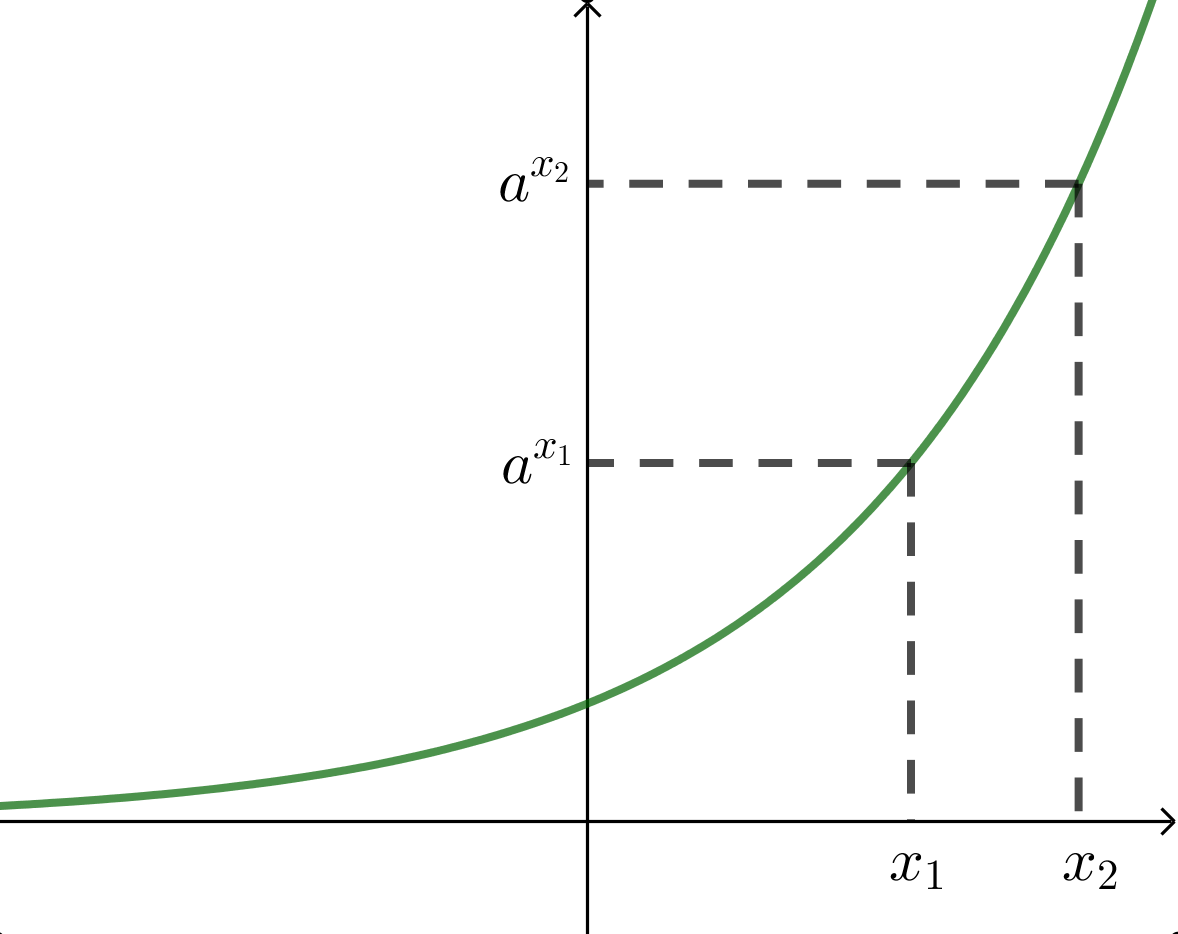
\includegraphics[width=0.4\textwidth]{inequality_1}
\qquad\quad
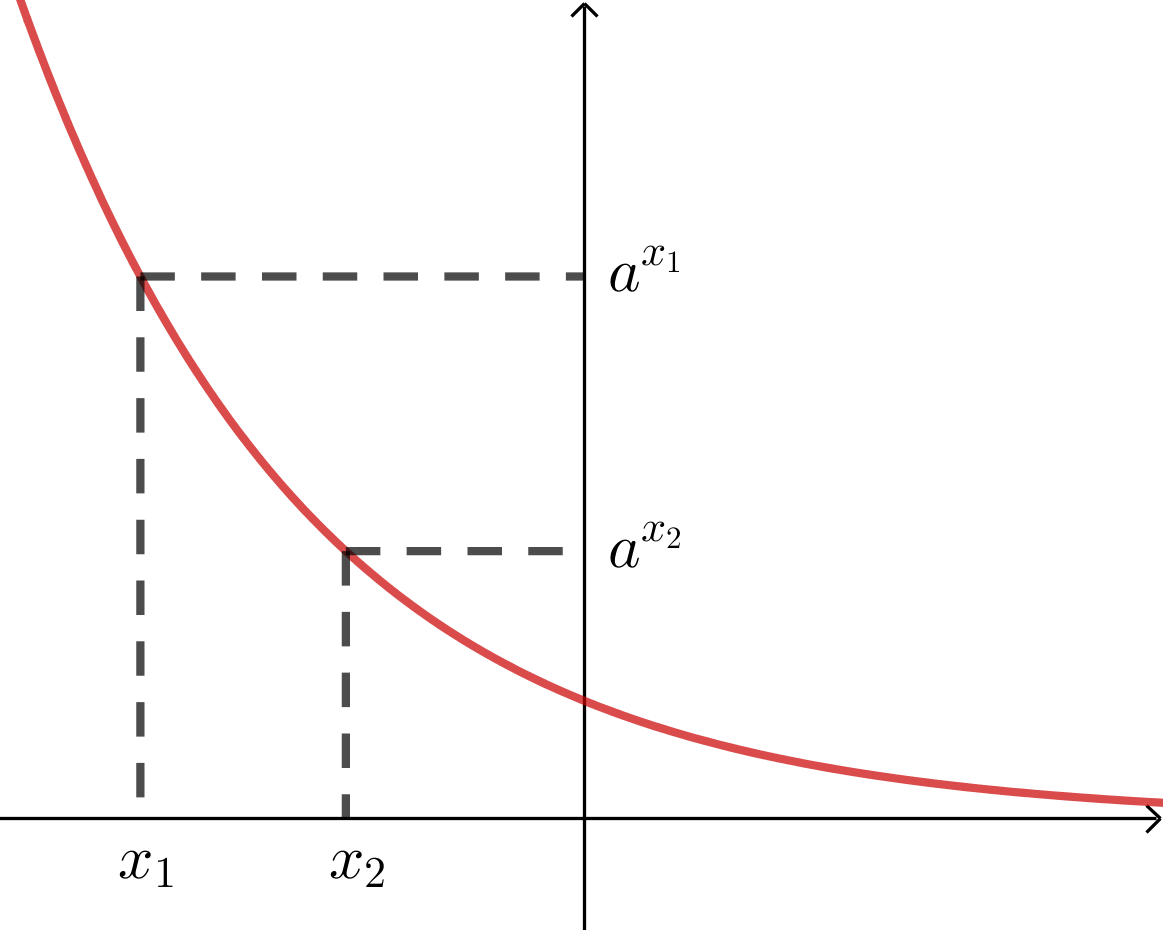
\includegraphics[width=0.4\textwidth]{inequality_2}
\begin{tabu}{X[c]X[c]}
\(a>1\)일 때
&
\(0<a<1\)일 때
\end{tabu}
\end{center}

%
\exam{\(0.04^x>0.2^{x+3}\)을 만족시키는 \(x\)의 범위를 구하여라.}\label{ineq1}
\begin{mdframed}
\(0.04=0.2^2\)이므로
\[0.2^{2x}>0.2^{x+3}\]
이다.
\(0<0.2<1\)이므로
\[2x<x+3\]
이다.
따라서 \(x<3\)이다.
\end{mdframed}
\ans{\(x<3\)}

%
\prob{다음 지수부등식을 푸시오.}\label{ineq2}
\begin{enumerate*}[itemjoin=\tabto{.5\textwidth}]
\item
\(25^x\ge625\)
\item
\(2^x>3\)
\end{enumerate*}

\newpage
로그부등식도 마찬가지의 방법으로 생각할 수 있다.
로그함수 \(y=\log_ax\)는 \(a>1\)일 때 증가함수, \(0<a<1\)일 때 감소함수이므로
\begin{mdframed}[leftmargin=.1\textwidth,rightmargin=.1\textwidth]\centering
\(a>1\)일 때,		\quad \(x_1<x_2\quad\Longleftrightarrow\quad \log_a{x_1}<\log_a{x_2}\)\\
\(0<a<1\)일 때,	\quad \(x_1<x_2\quad\Longleftrightarrow\quad \log_a{x_1}>\log_a{x_2}\)
\end{mdframed}
\begin{center}
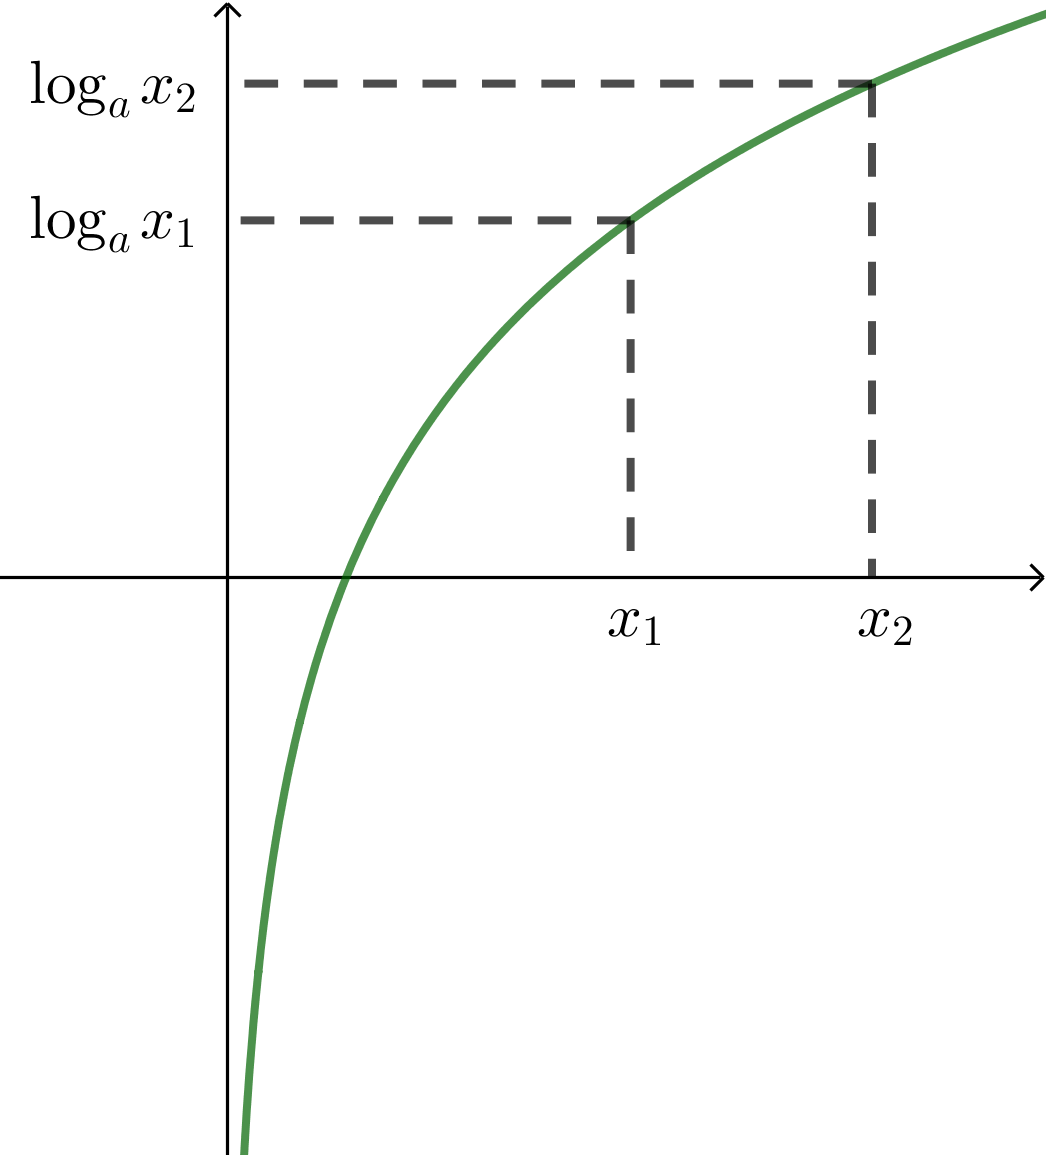
\includegraphics[width=0.4\textwidth]{inequality_3}
\qquad\quad
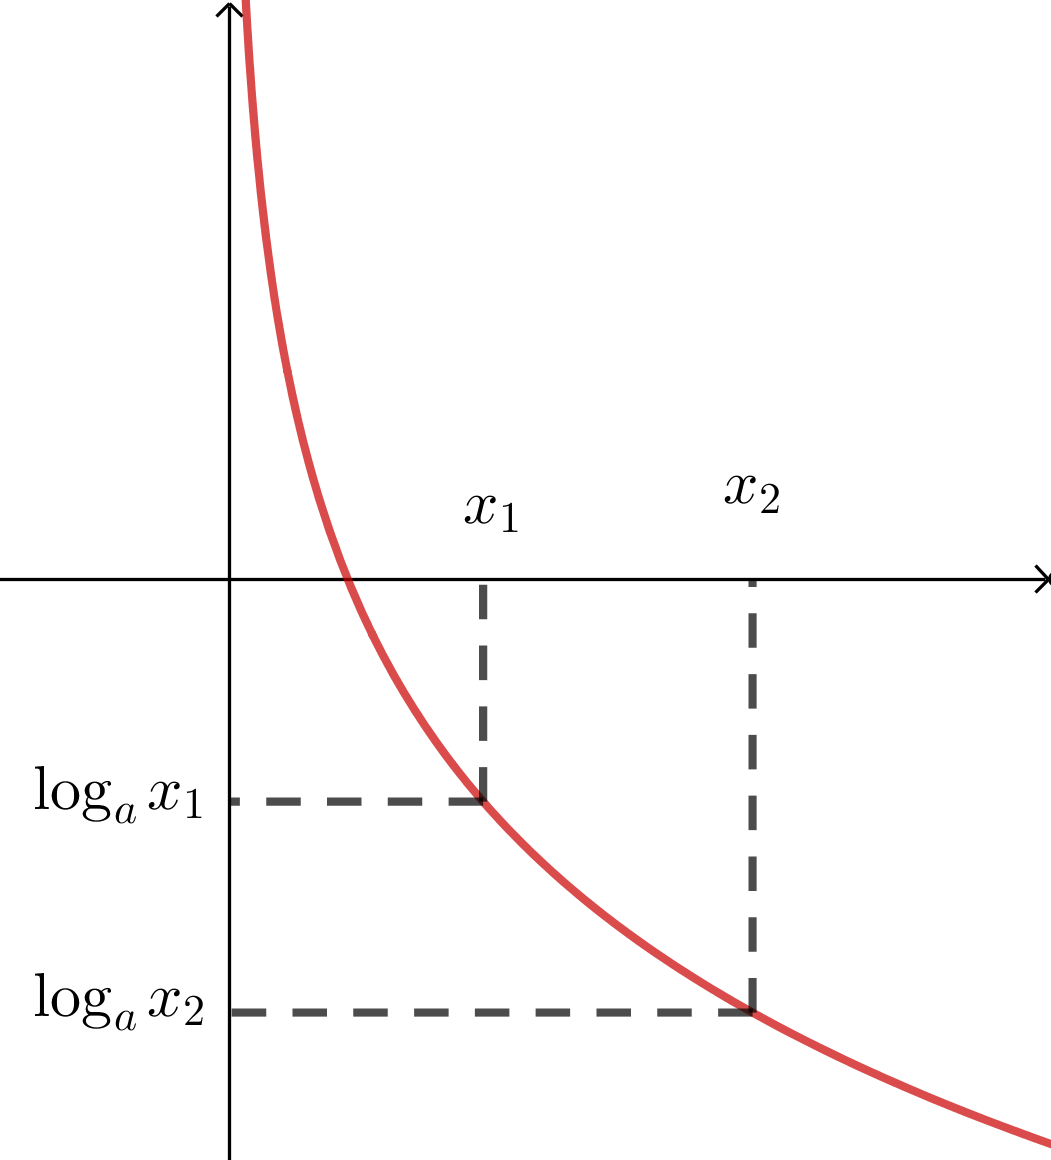
\includegraphics[width=0.4\textwidth]{inequality_4}
\begin{tabu}{X[c]X[c]}
\(a>1\)일 때
&
\(0<a<1\)일 때
\end{tabu}
\end{center}
%로그부등식을 풀 때에도 진수 조건에 유의하여 푼다.

%
\exam{\(\log_2x+\log_2(x-1)<1\)을 만족시키는 \(x\)값의 범위를 구하여라.}\label{ineq3}
\\[-20pt]
\begin{mdframed}
주어진 식의 좌변과 우변을 각각 변형하면
\(\log_2(x^2-x)<\log_22\)
가 된다.
따라서 \(x^2-x<2\), \(x^2-x-2<0\), \((x-2)(x+1)<0\)이므로
\[-1<x<2\tag{1}\]
이다.
이때, 진수는 0보다 커야하므로 \(x>0\), \(x-1>0\)이다.
두 부등식을 연립하면
\[x>1\tag{2}\]
이므로, (1)과 (2)를 연립하면 \(1<x<2\)가 된다.
\end{mdframed}
\ans{\(1<x<2\)}

%
\prob{다음 로그부등식을 푸시오.}\label{ineq4}
\begin{enumerate*}[itemjoin=\tabto{.5\textwidth}]
\item
\(\log_3(2x-1)\le2\)
\item
\(\log_{\frac13}(x-1)>\log_{\frac13}(7-x)\)
\end{enumerate*}

%%%
\section*{답}
\addcontentsline{toc}{chapter}{\protect\numberline{*}답}
\begin{multicols*}{2}
%
\an{review2}
\begin{center}
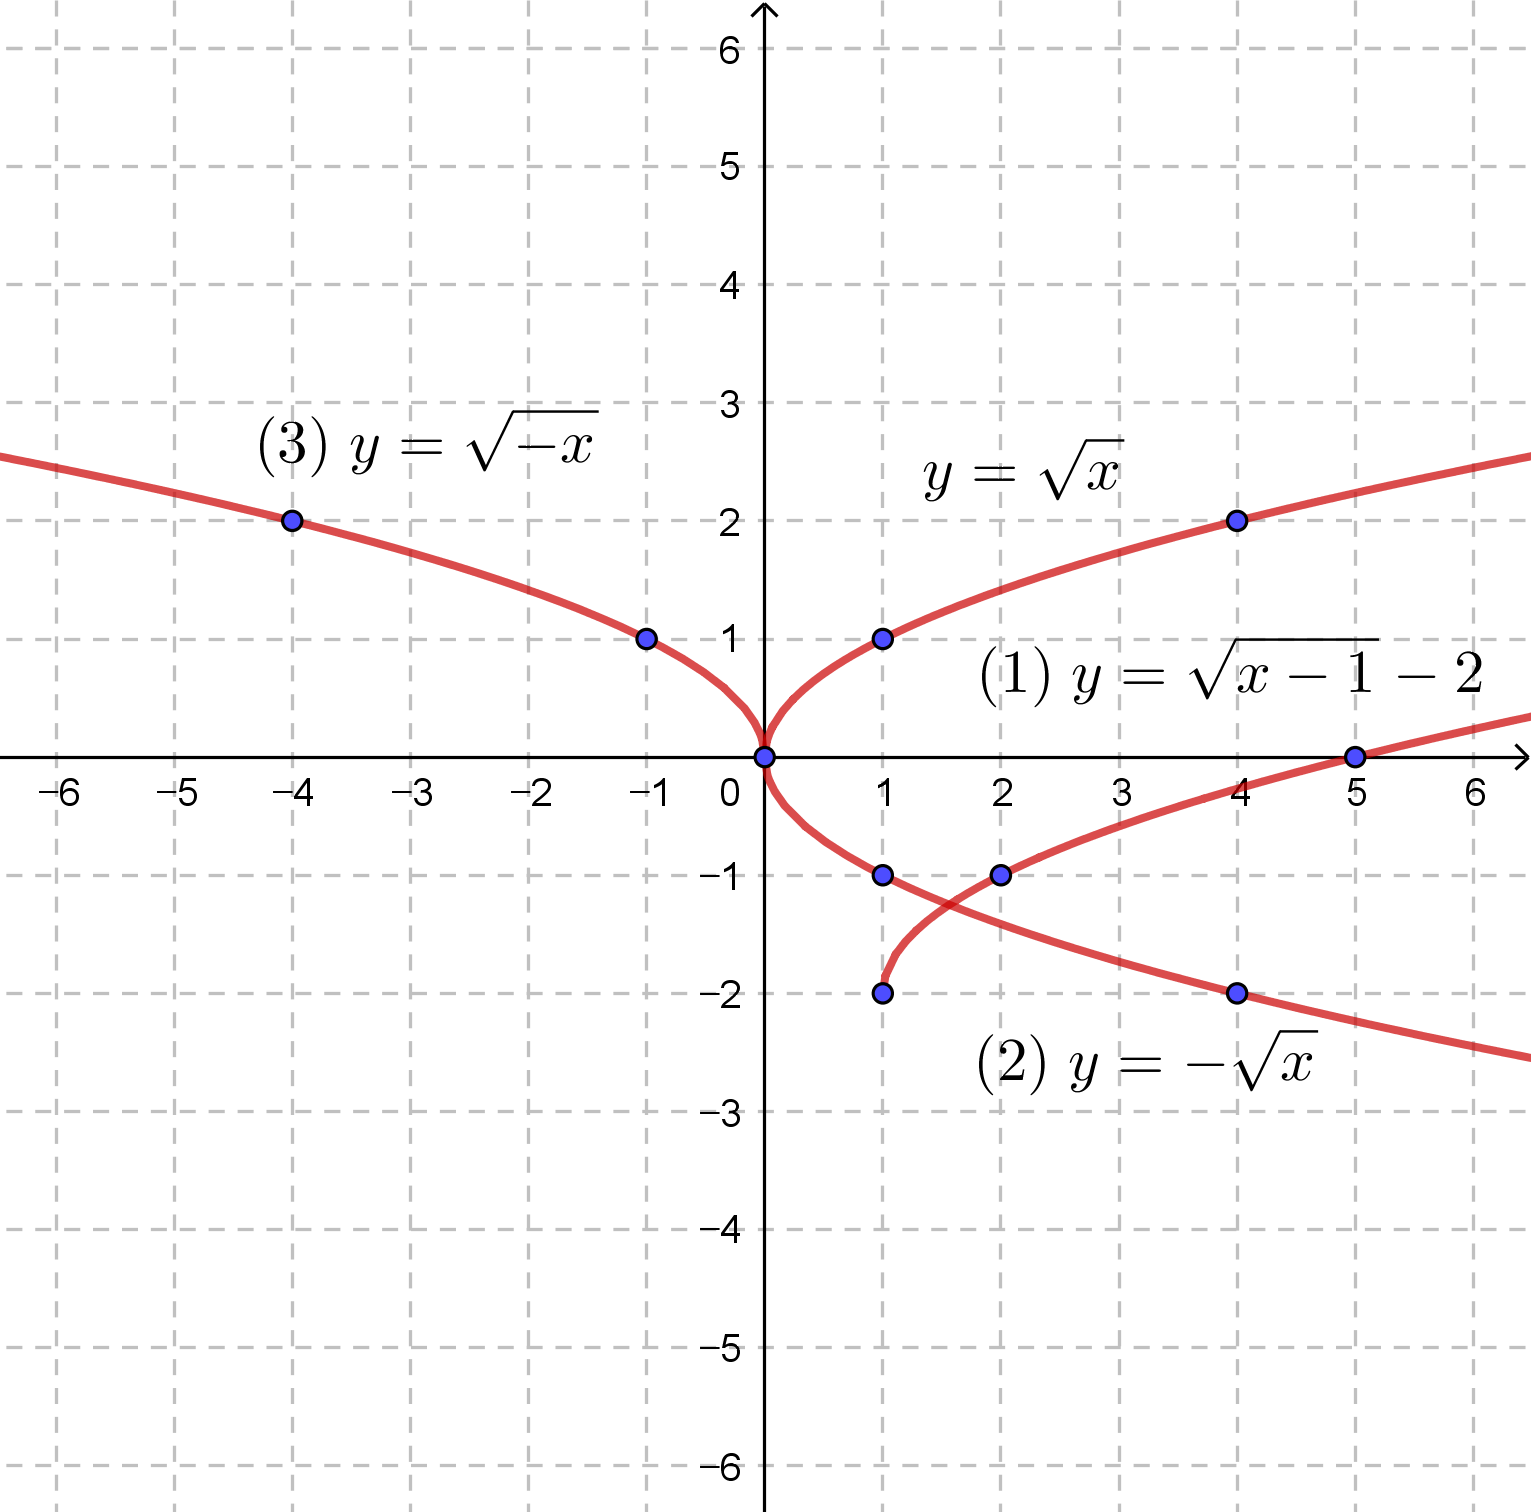
\includegraphics[width=\columnwidth]{review_2}
\end{center}

%
\ann{review4}{\(a=2\), \(b=1\), \(c=0\)}

%
\an{review7}
\begin{enumerate}
\item
증가
\item
증가
\item
감소, 증가
\end{enumerate}

%
\an{review8}
\begin{enumerate}
\item
\(\frac12x-2\)
\item
\(\{y\ba y\neq3\}\)
\item
\(\{x\ba x\ge2\}\)
\end{enumerate}

%
\an{review9}
\begin{enumerate*}[itemjoin=\quad]
\item
125
\item
60
\item
10
\item
10
\end{enumerate*}

\columnbreak
%
\an{exp2}
\begin{center}
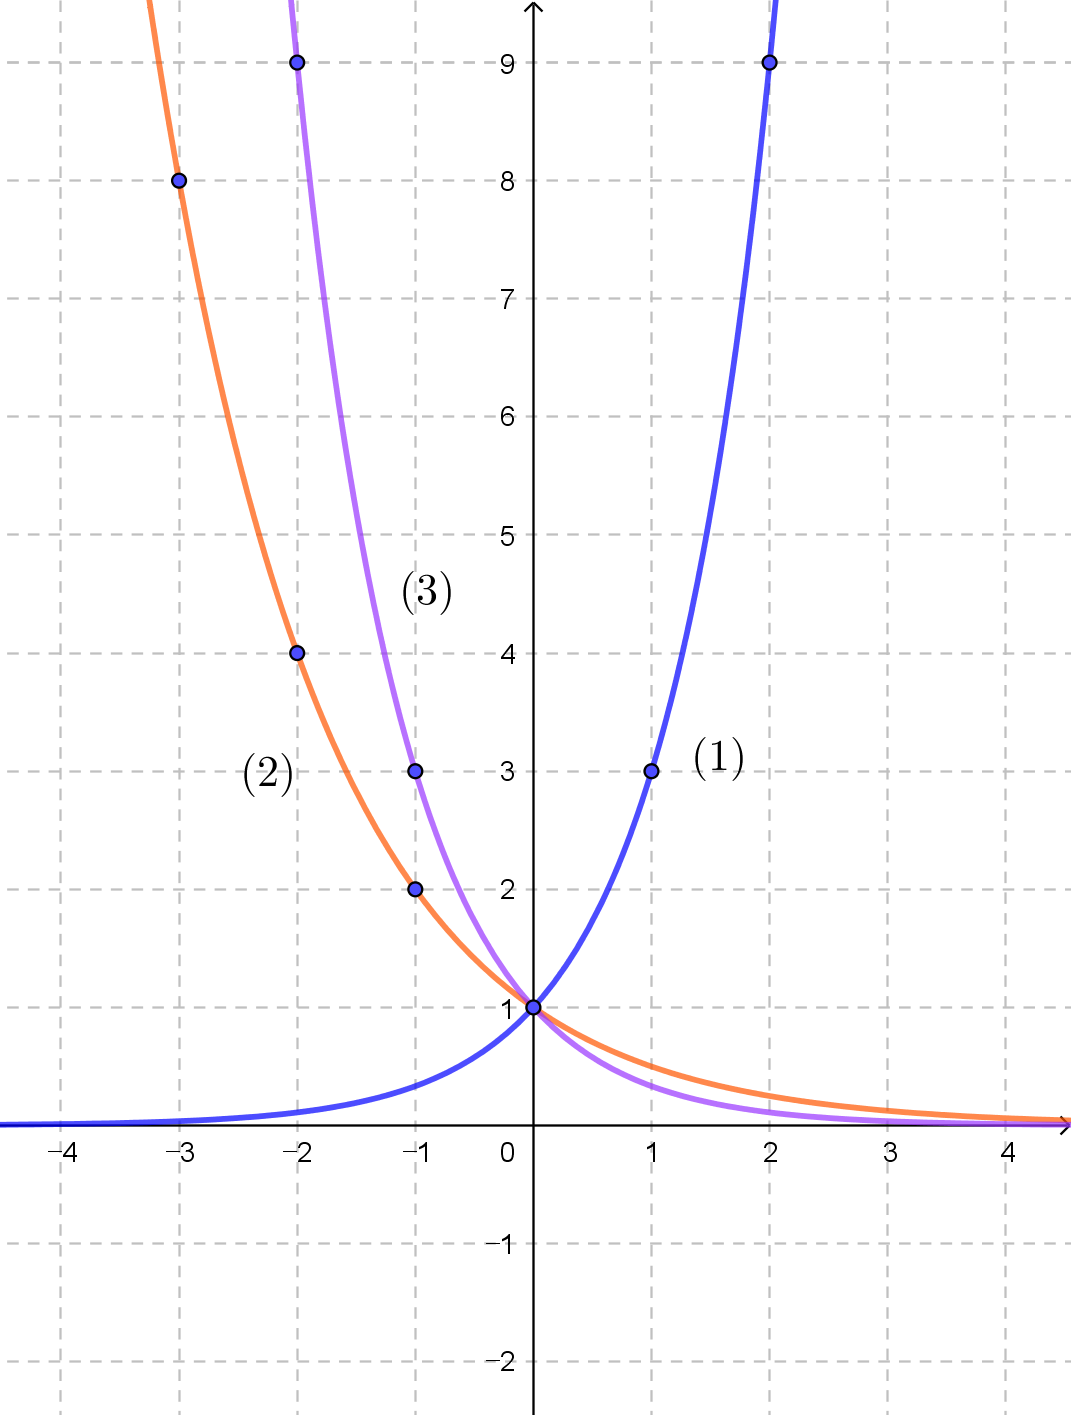
\includegraphics[width=0.8\columnwidth]{exp_2}
\end{center}

%
\an{exp5}
\begin{center}
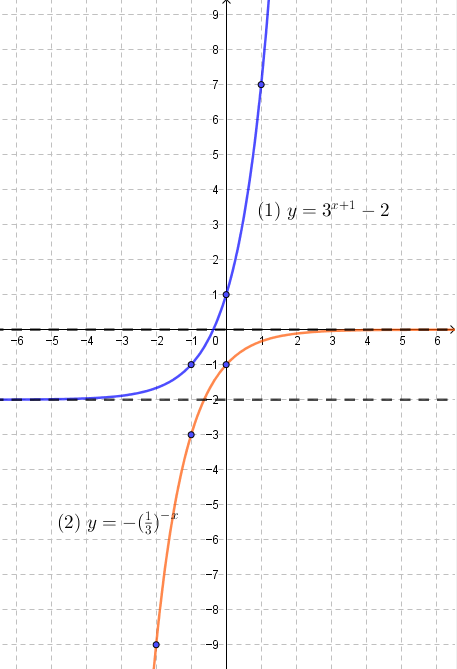
\includegraphics[width=\columnwidth]{exp_5}
\end{center}
점근선 : (1) \(y=-2\), (2) \(y=0(x축)\)

\columnbreak
%
\ann{log2}{\four}

%
\an{log3}
\begin{center}
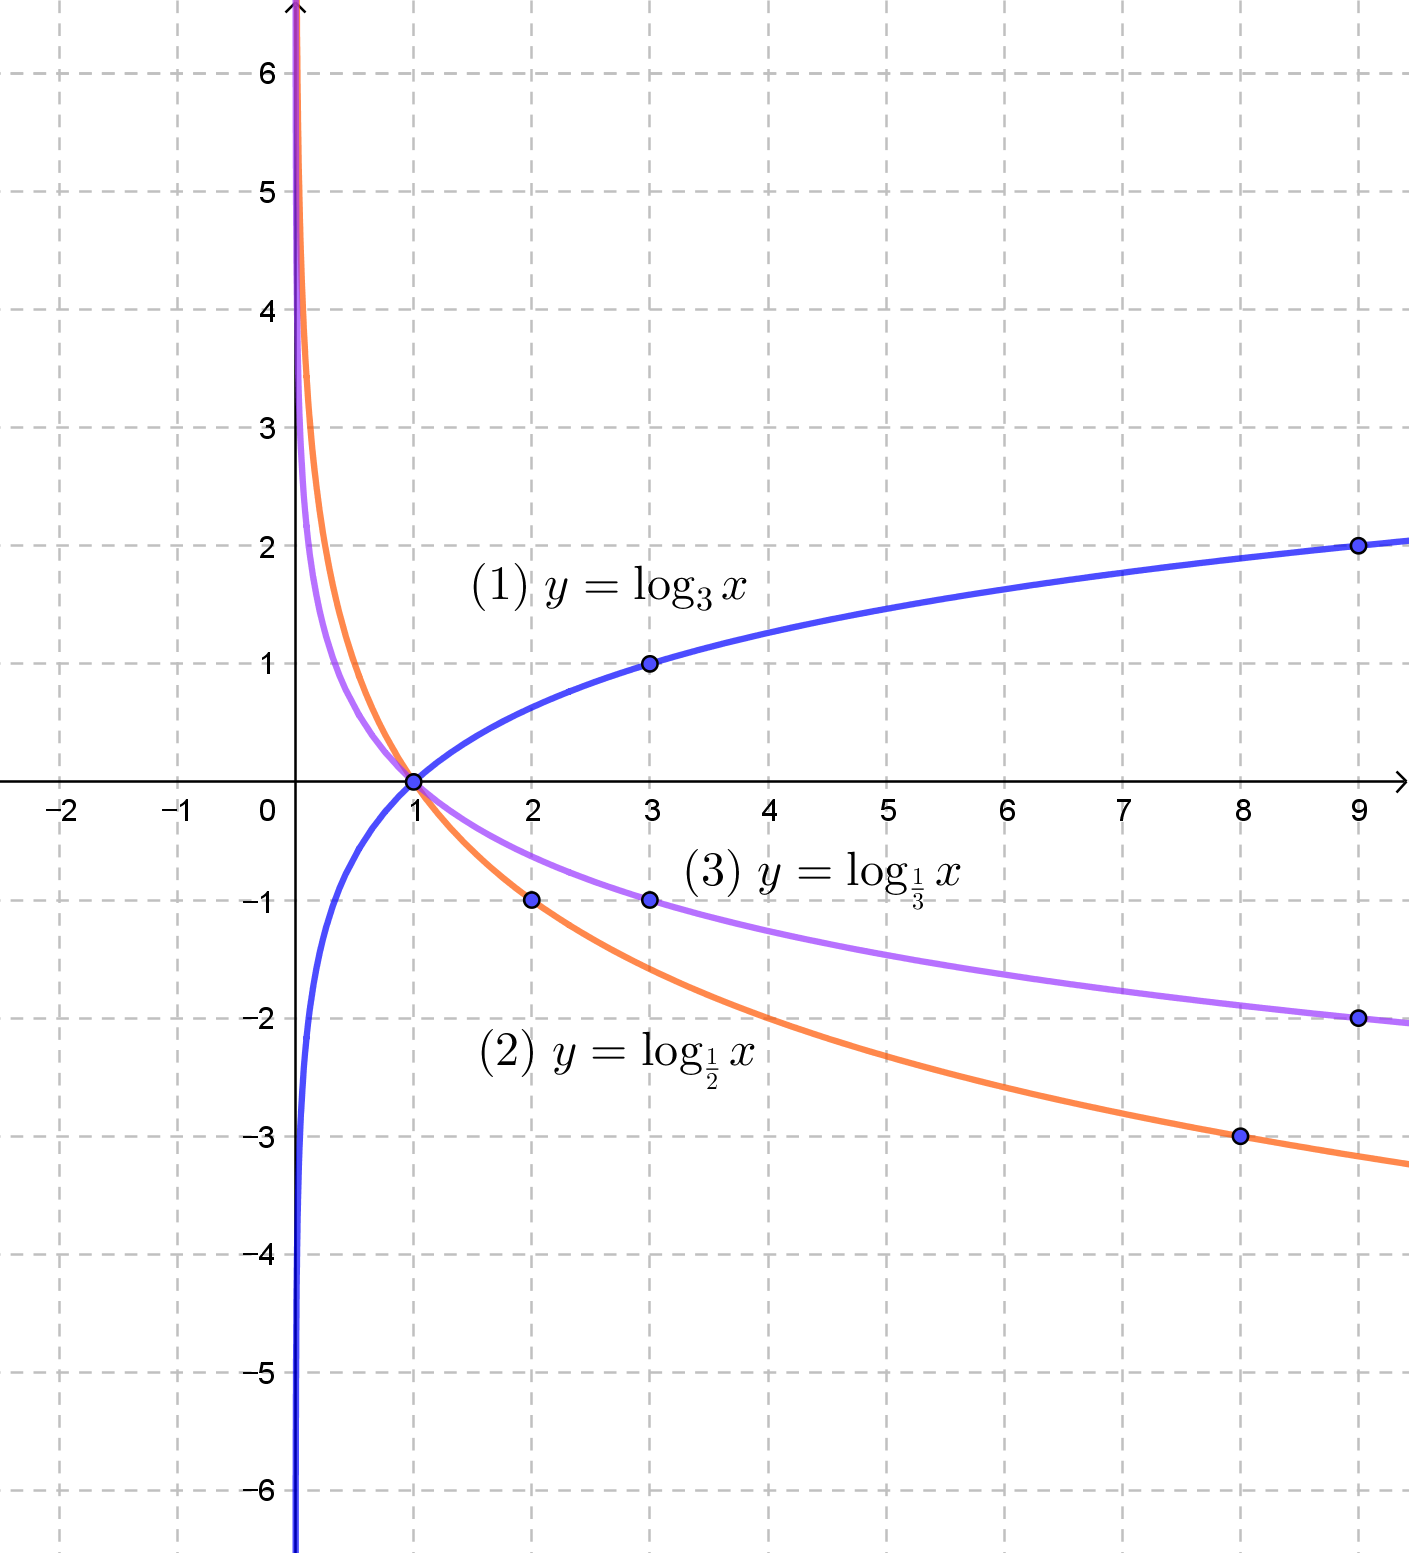
\includegraphics[width=\columnwidth]{log_3}
\end{center}

%
\an{log6}
(1) 점근선 : \(x=-1\)
\begin{center}
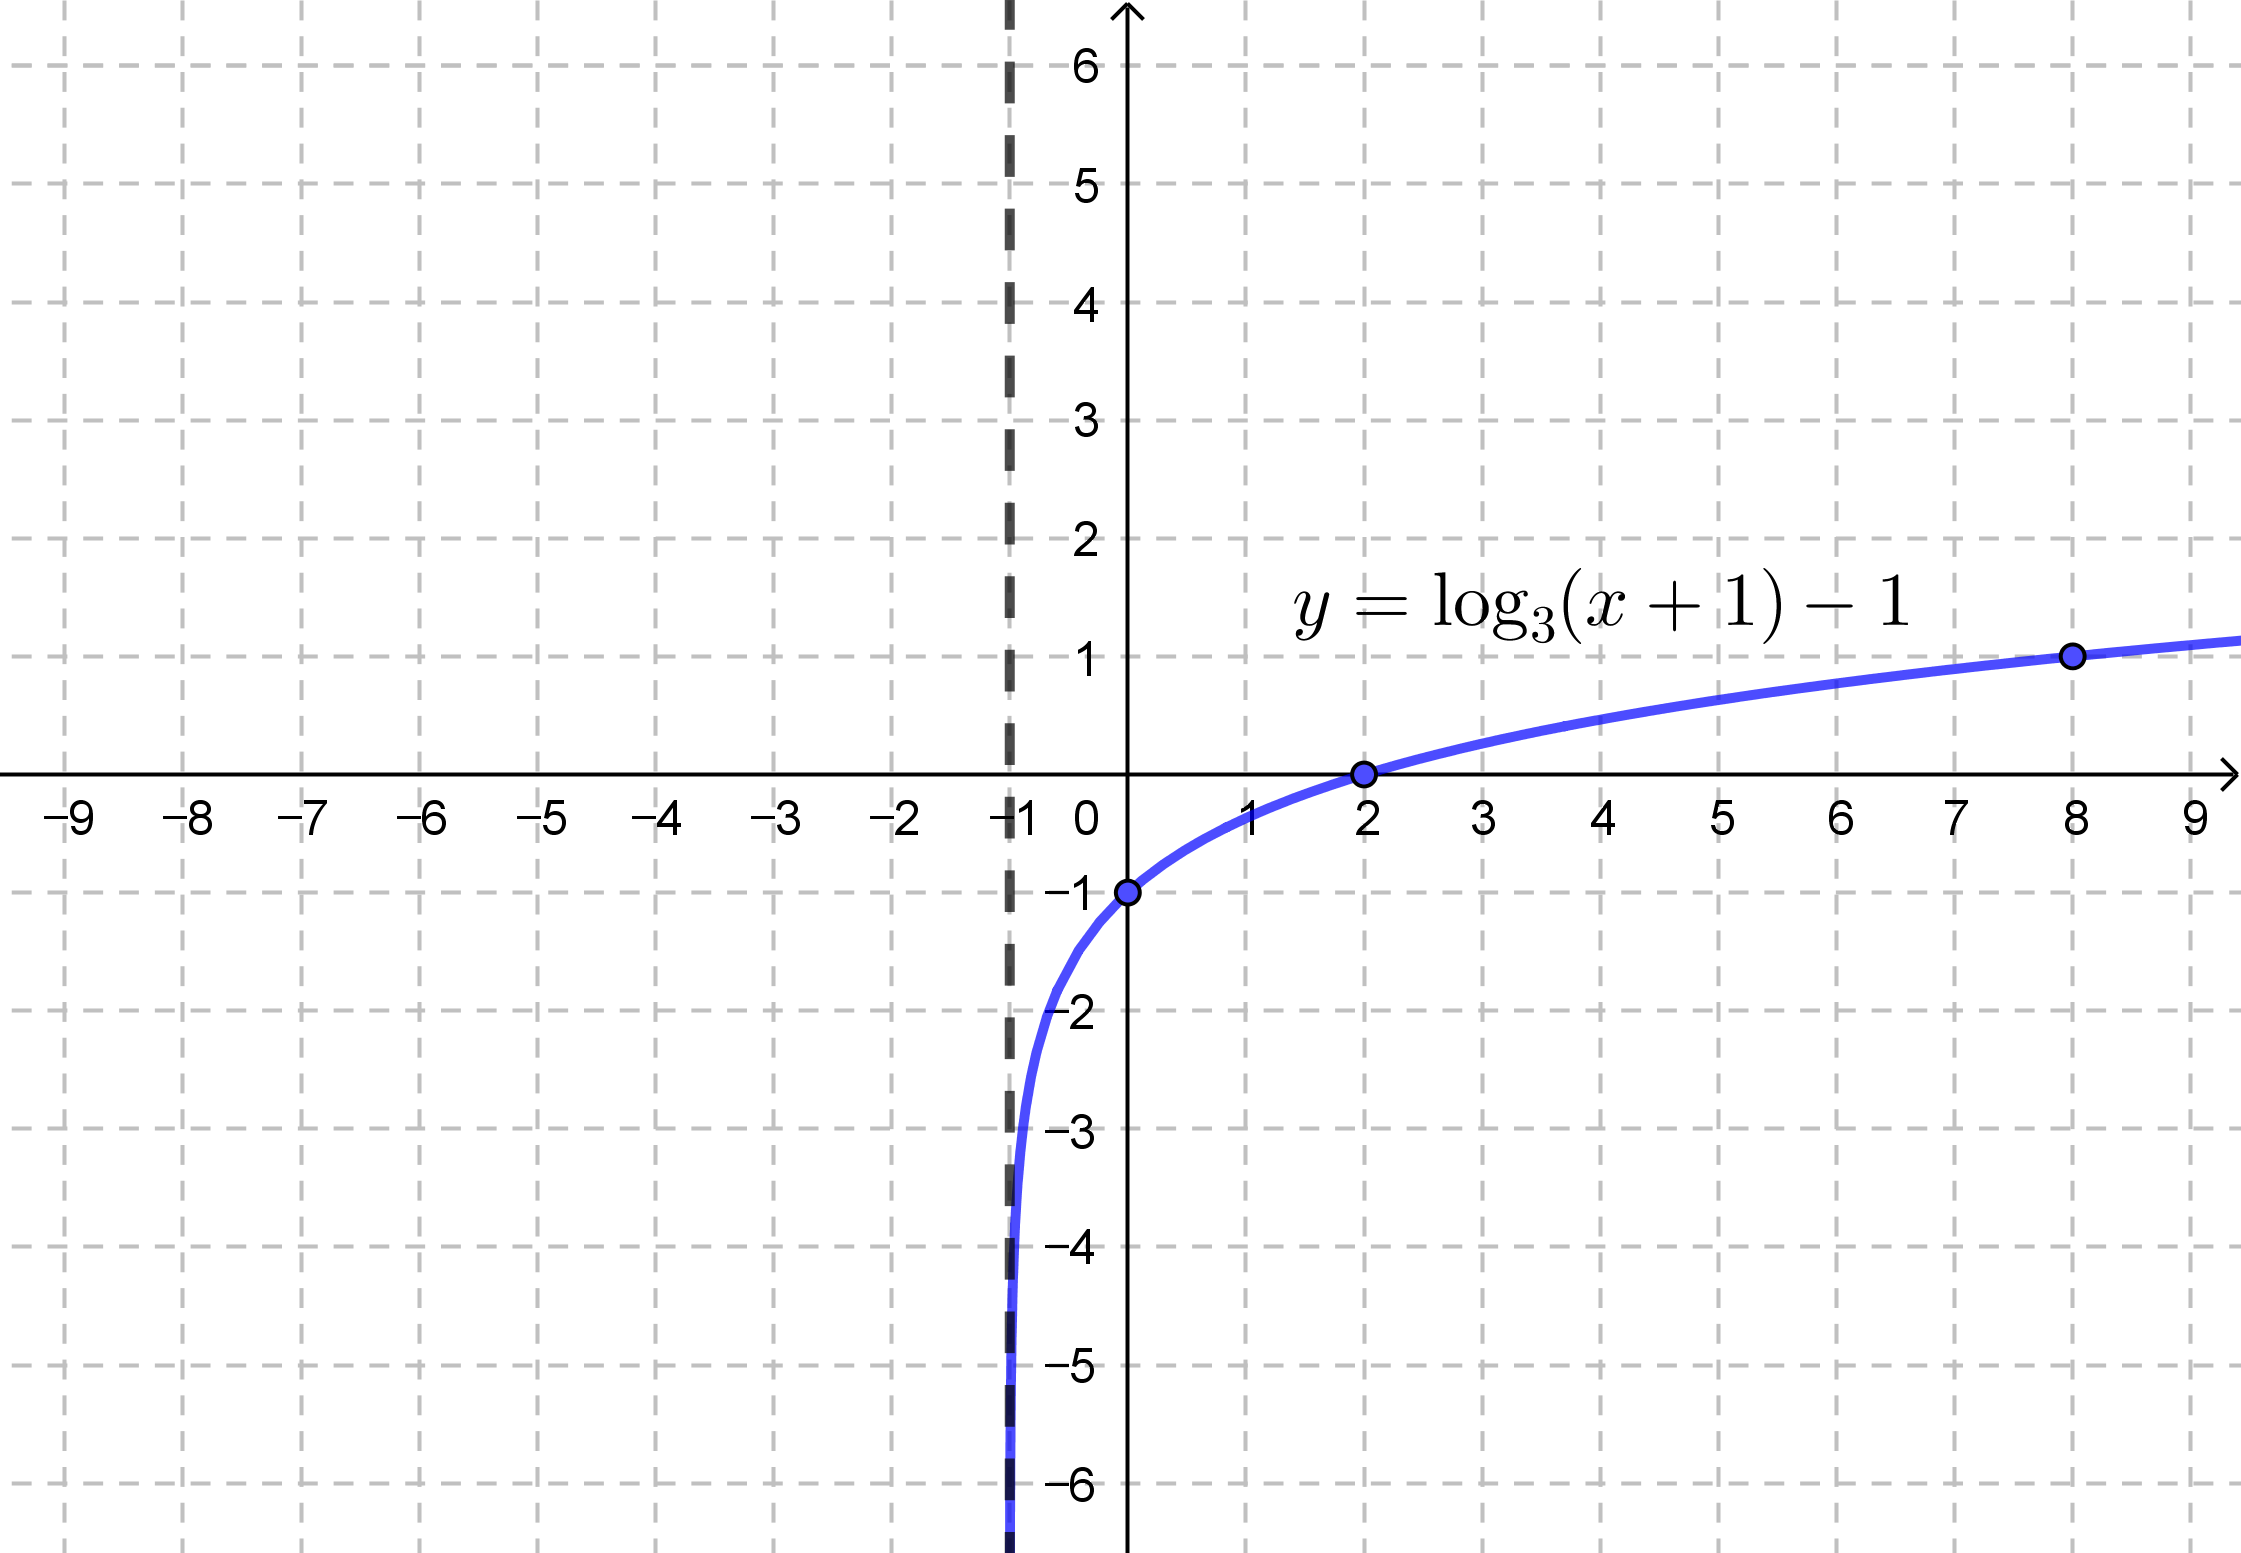
\includegraphics[width=\columnwidth]{log_6-1}
\end{center}
\par\noindent
(2) 점근선 : \(x=0(y축)\)
\begin{center}
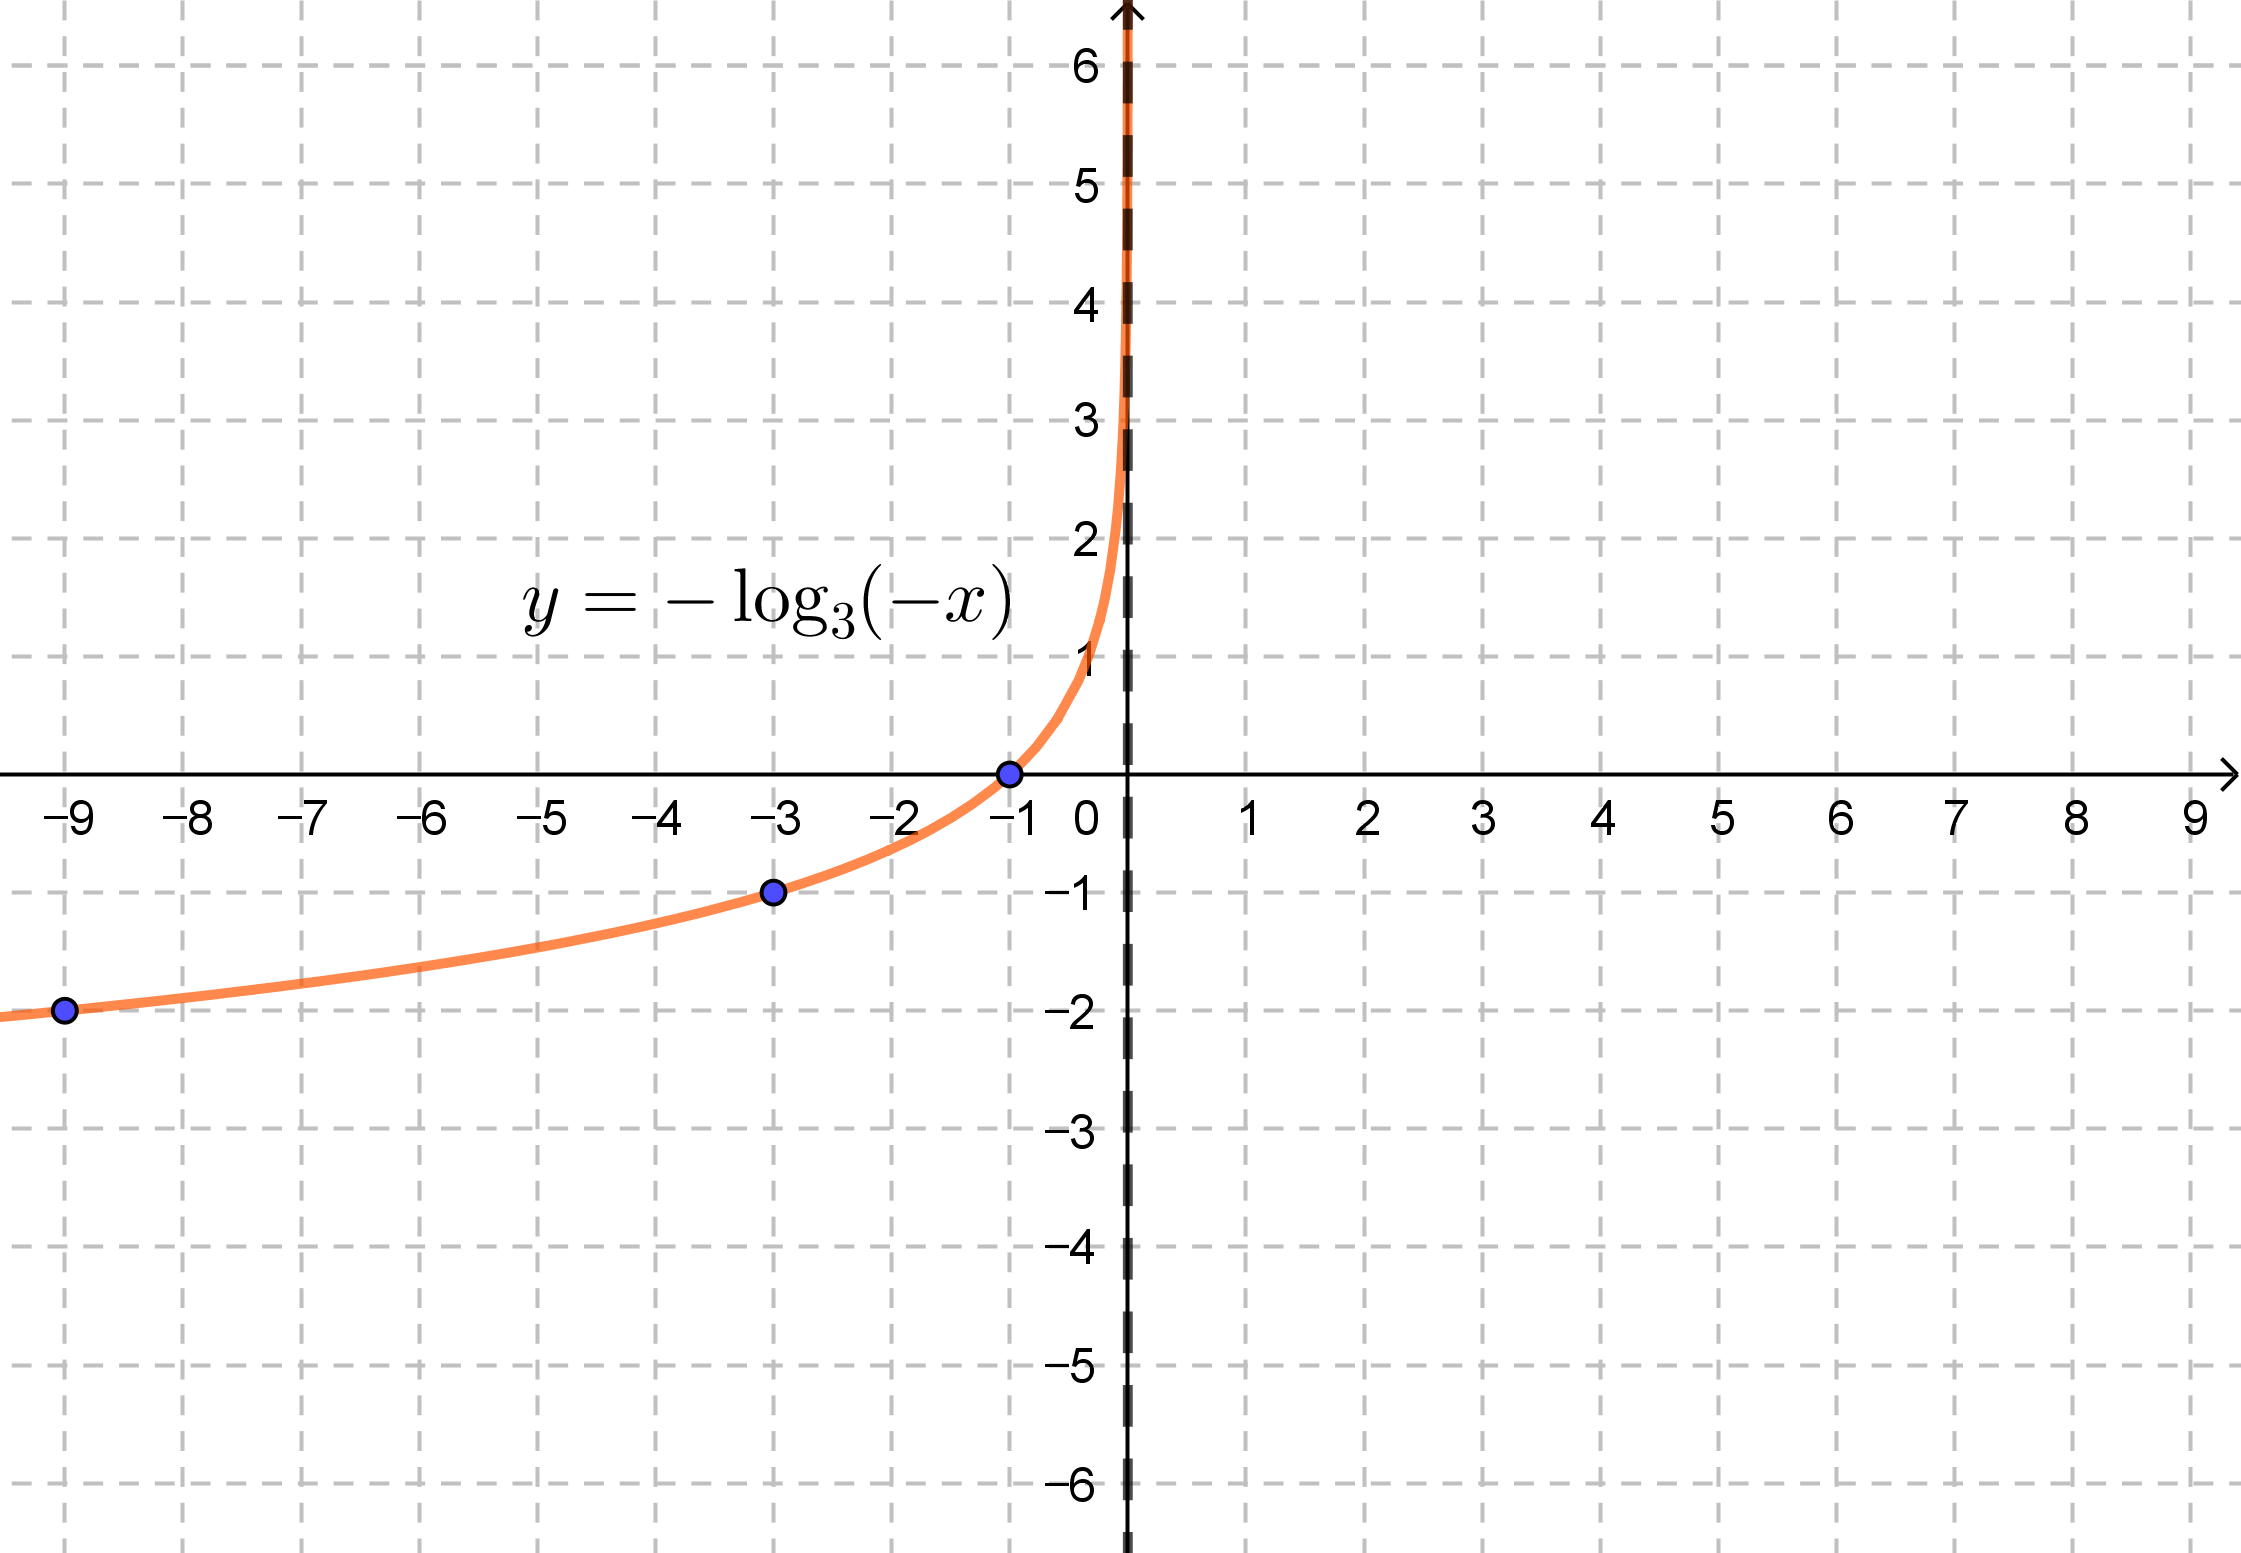
\includegraphics[width=\columnwidth]{log_6-2}
\end{center}

%
\an{equa2}
\begin{enumerate}
\item
\(x=\frac12\)
\item
\(x=-\frac52\)
\end{enumerate}

%
\an{equa4}
\begin{enumerate}
\item
\(x=7\)
\item
\(x=\frac12\)
\end{enumerate}

%
\an{ineq2}
\begin{enumerate}
\item
\(x\ge2\)
\item
\(x>\log_23\)
\end{enumerate}

%
\an{ineq4}
\begin{enumerate}
\item
\(\frac12<x\le5\)
\item
\(1<x<4\)
\end{enumerate}
\end{multicols*}

%
\section*{요약}
\addcontentsline{toc}{chapter}{\protect\numberline{*}요약}
\begin{enumerate}[label=\arabic*.,itemsep=40pt]
\item
지수함수의 그래프
\begin{center}
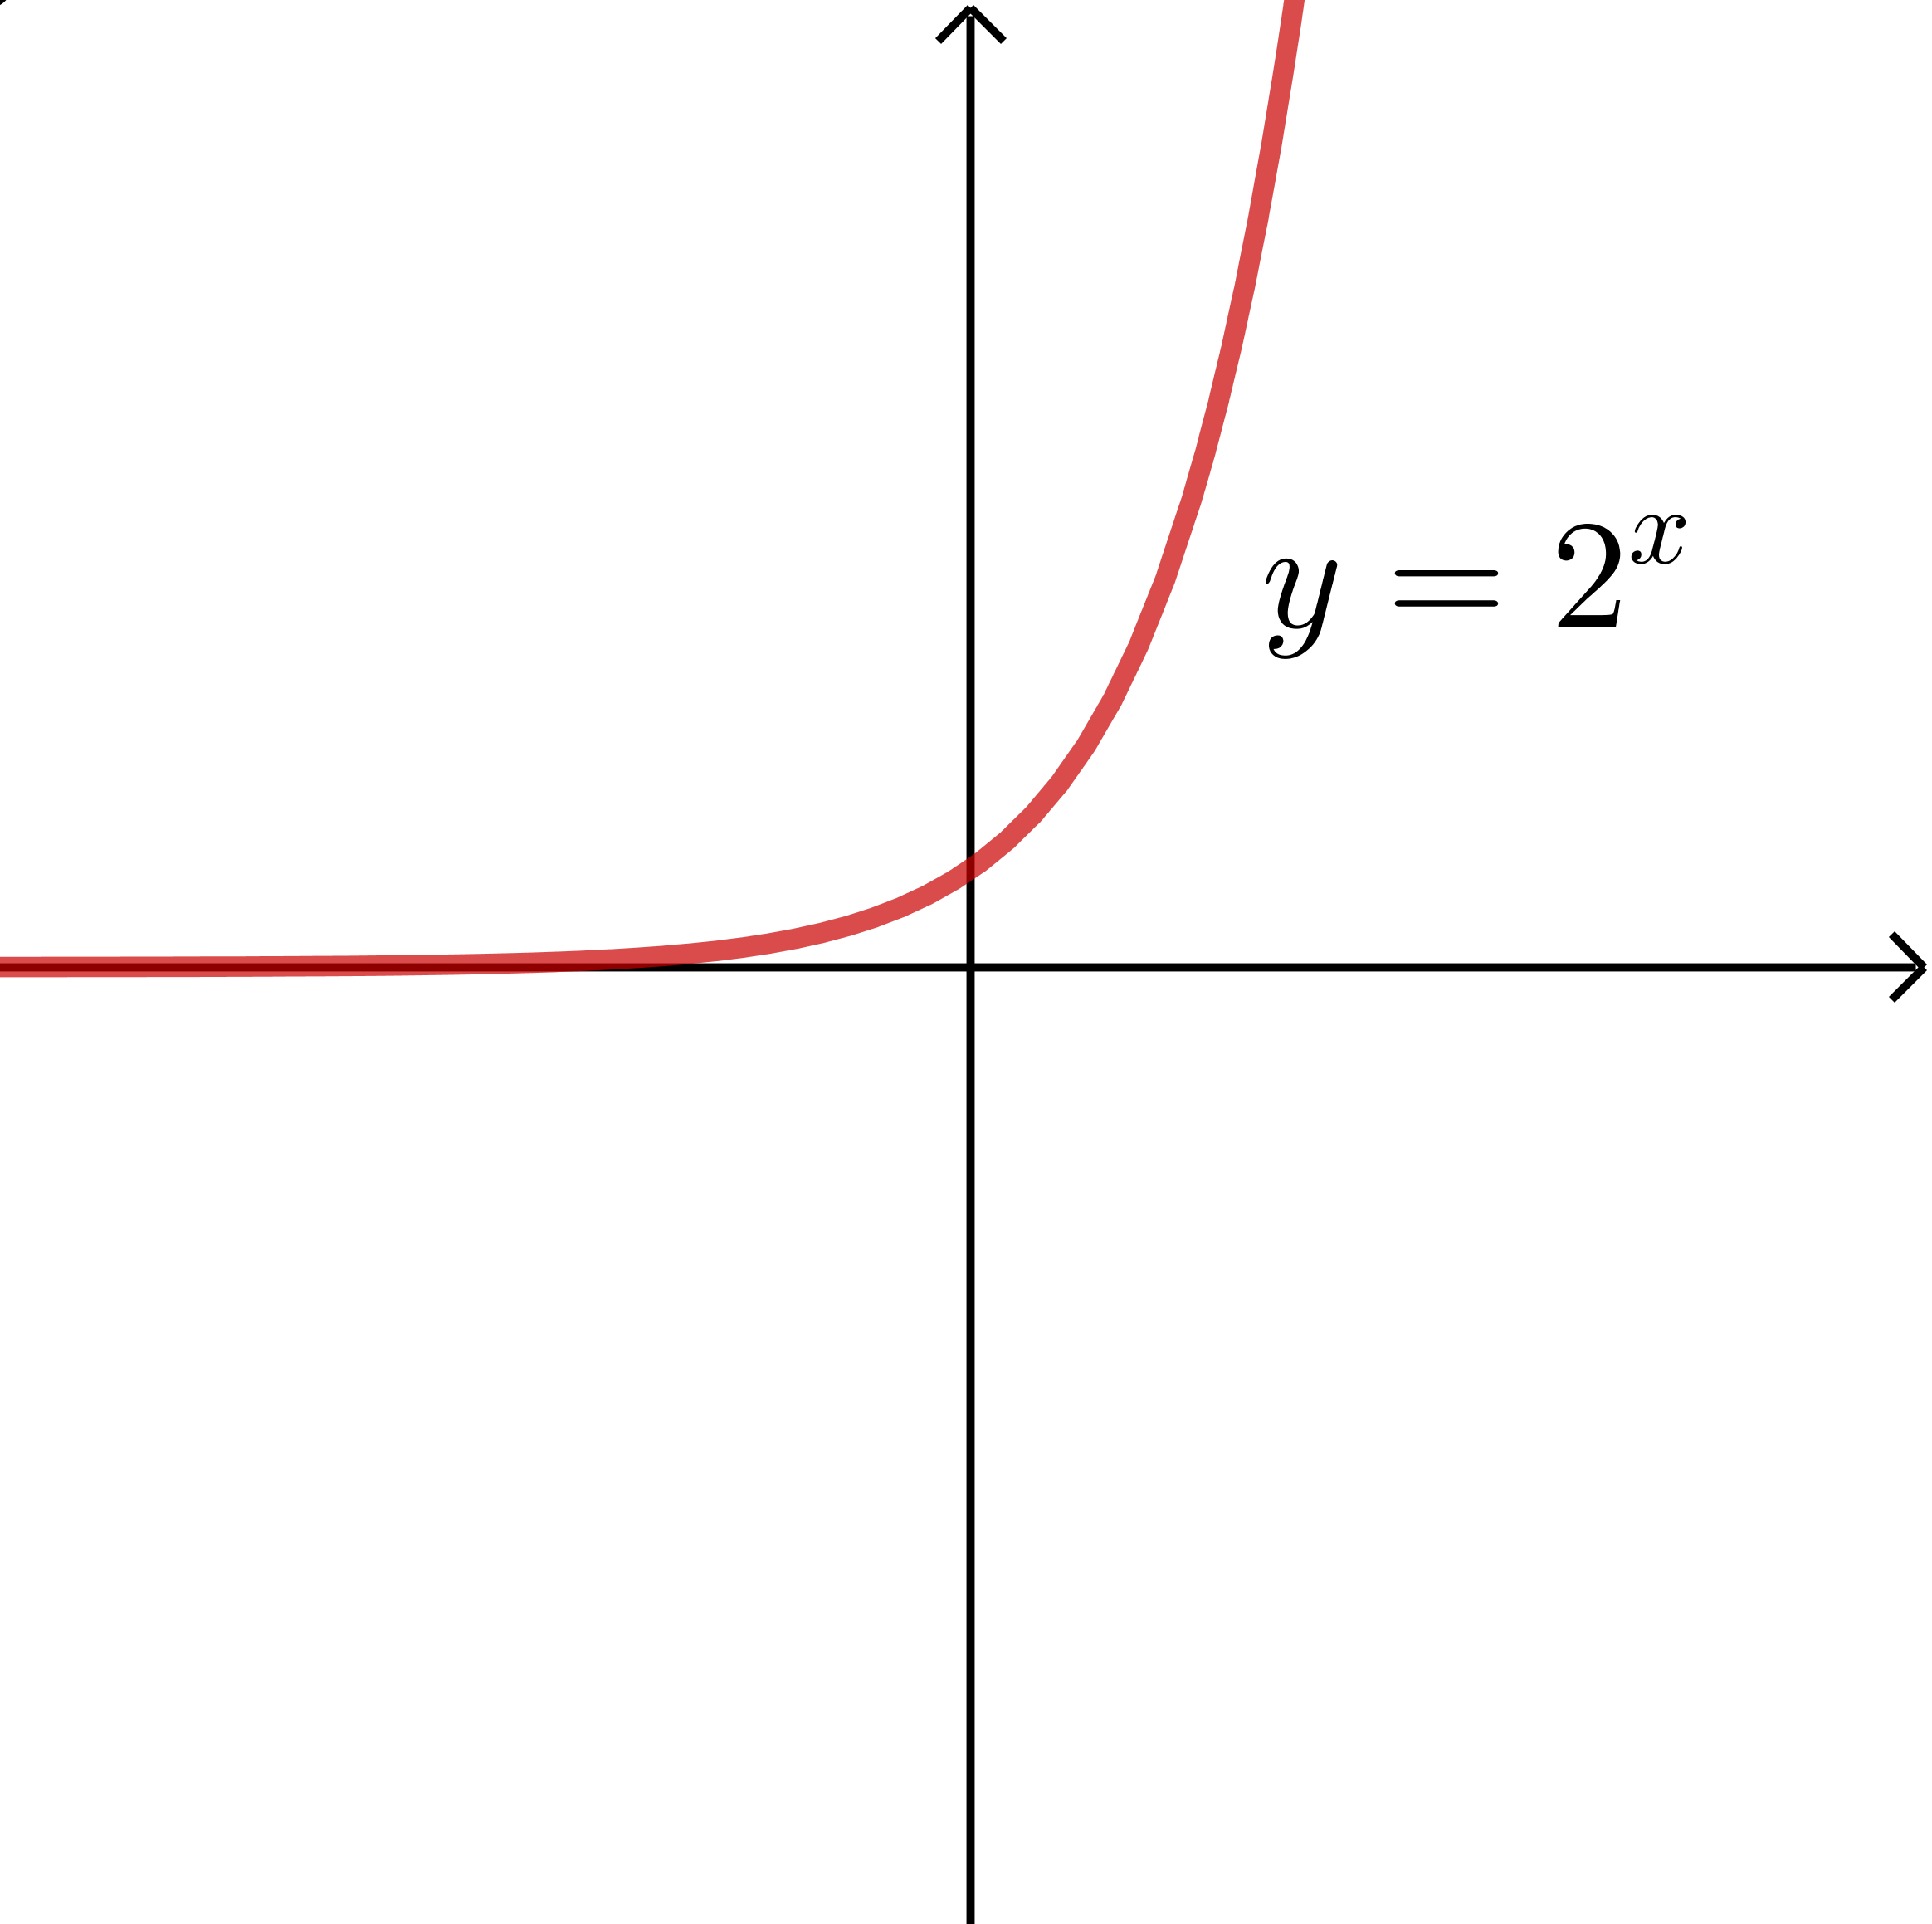
\includegraphics[width=0.3\textwidth]{summary_1}
\qquad\quad
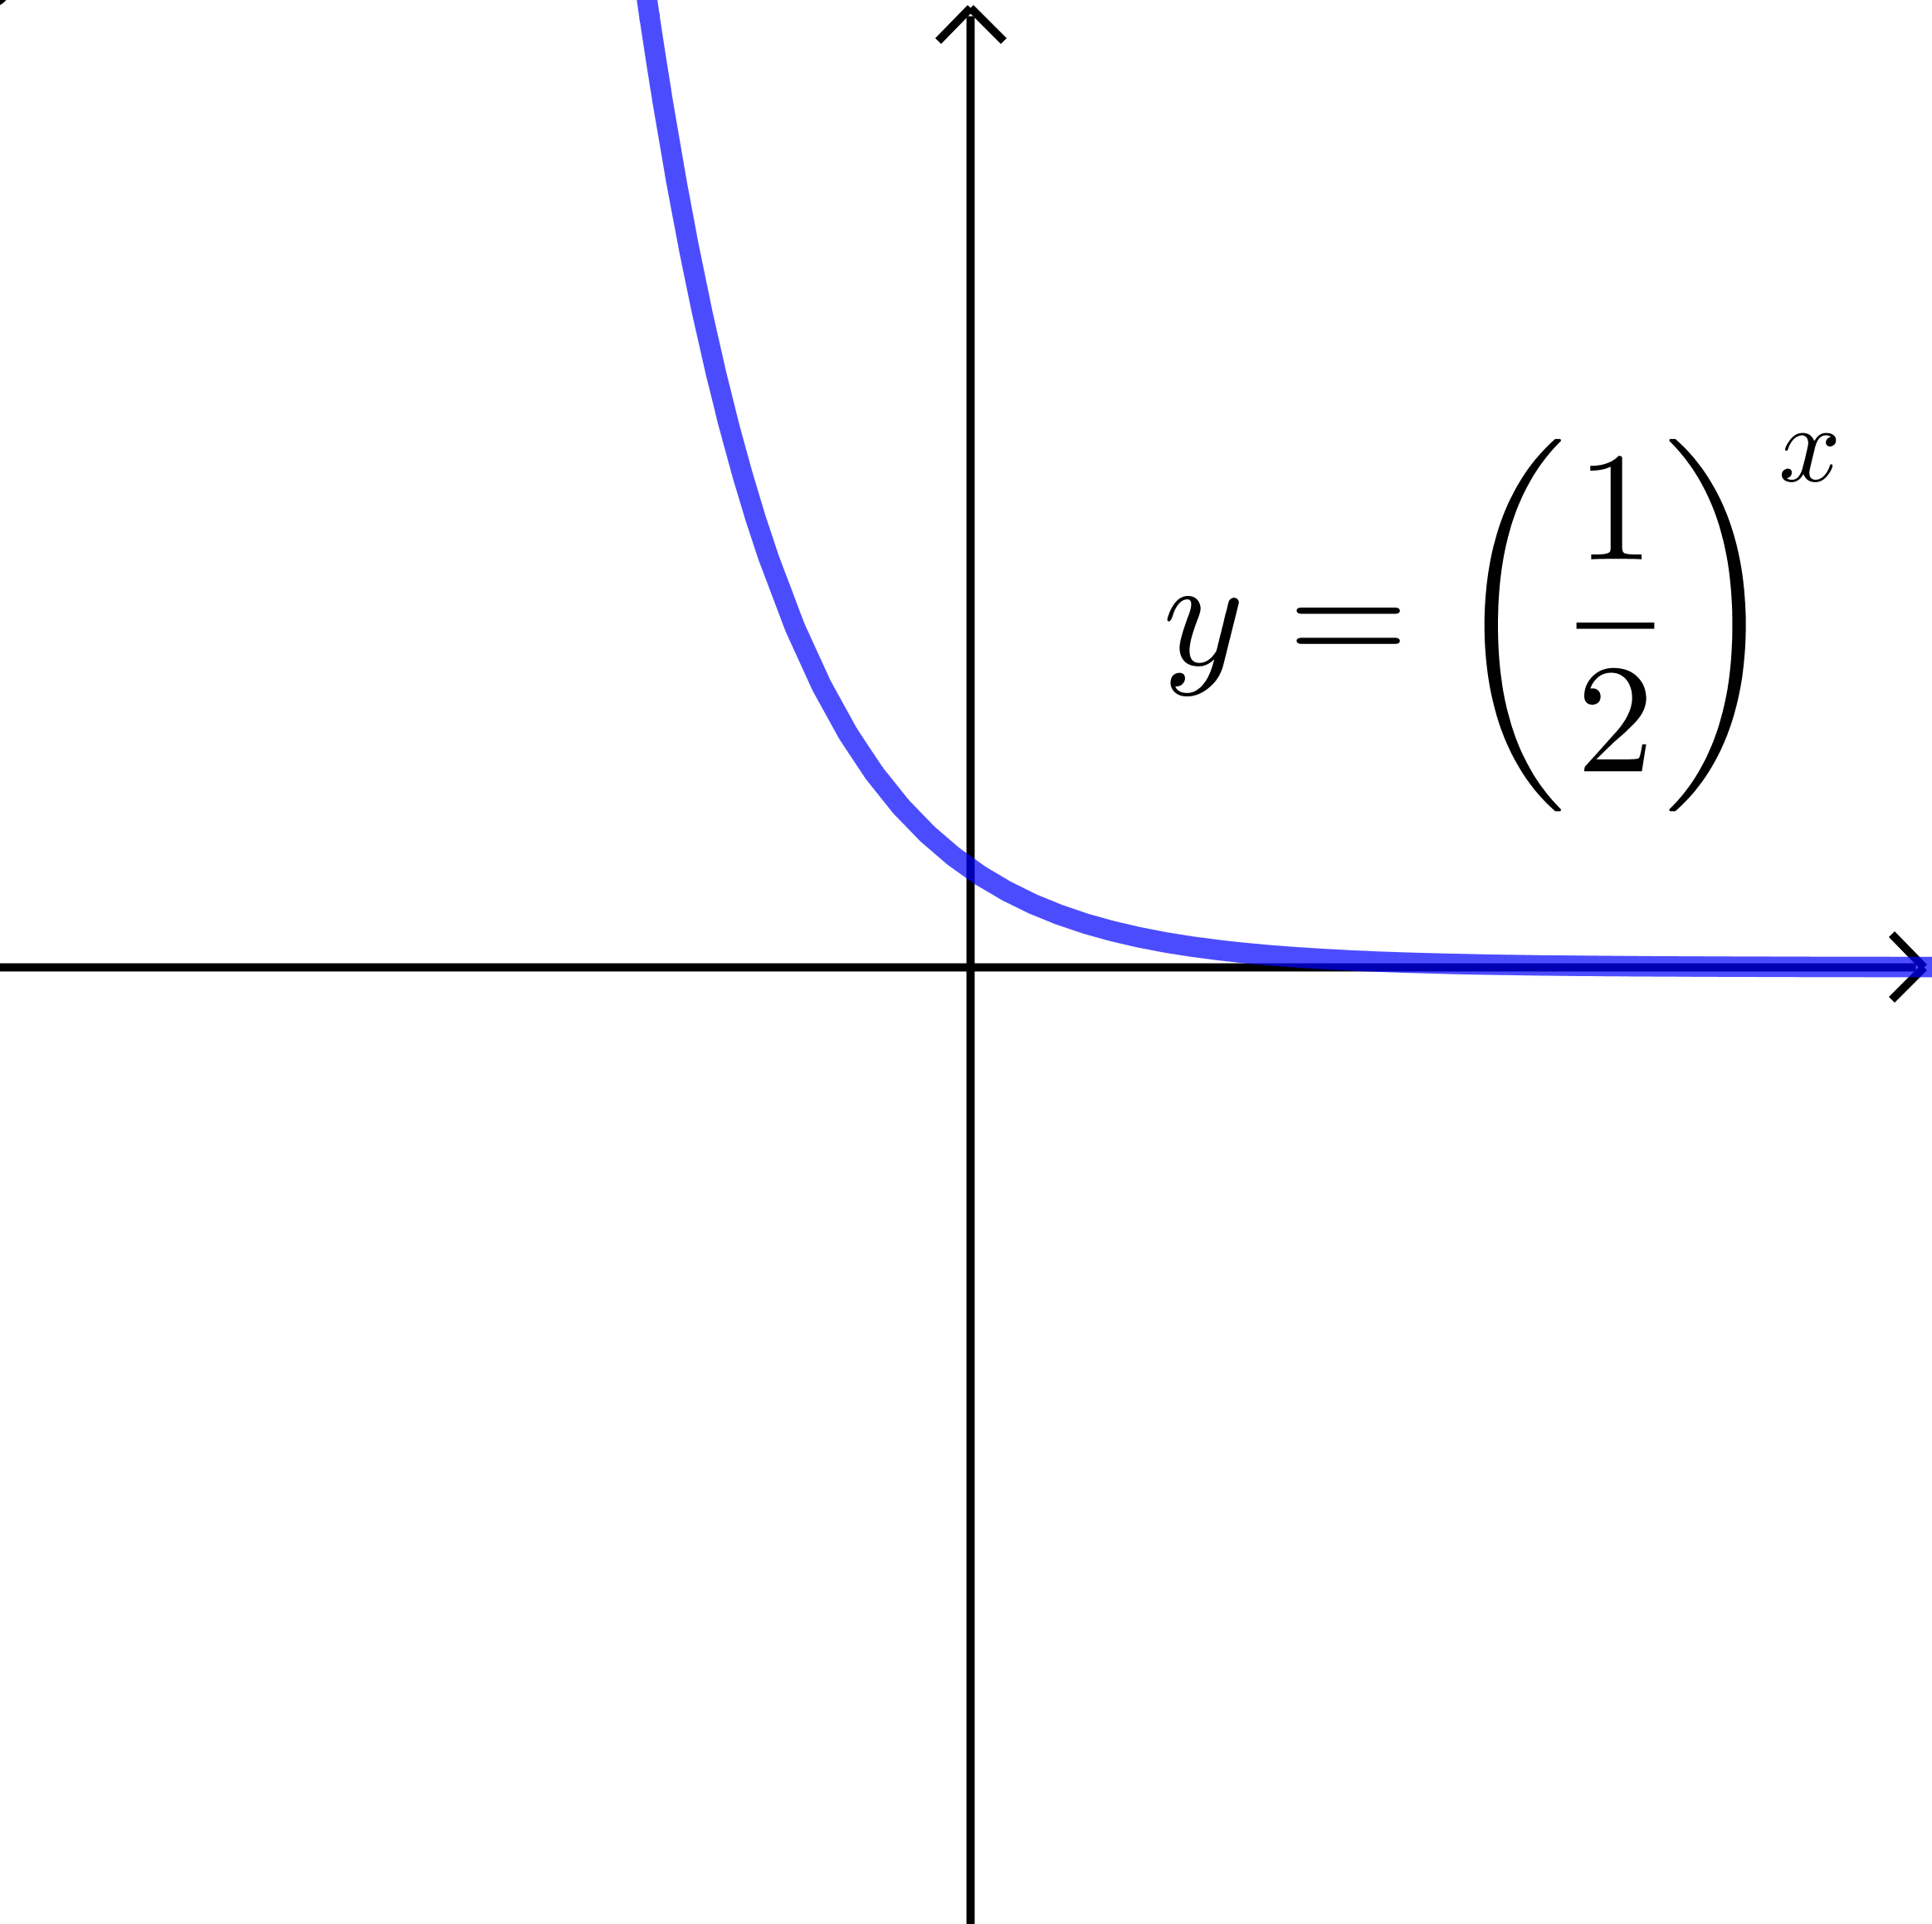
\includegraphics[width=0.3\textwidth]{summary_2}
\end{center}
\item
로그함수의 그래프
\begin{center}
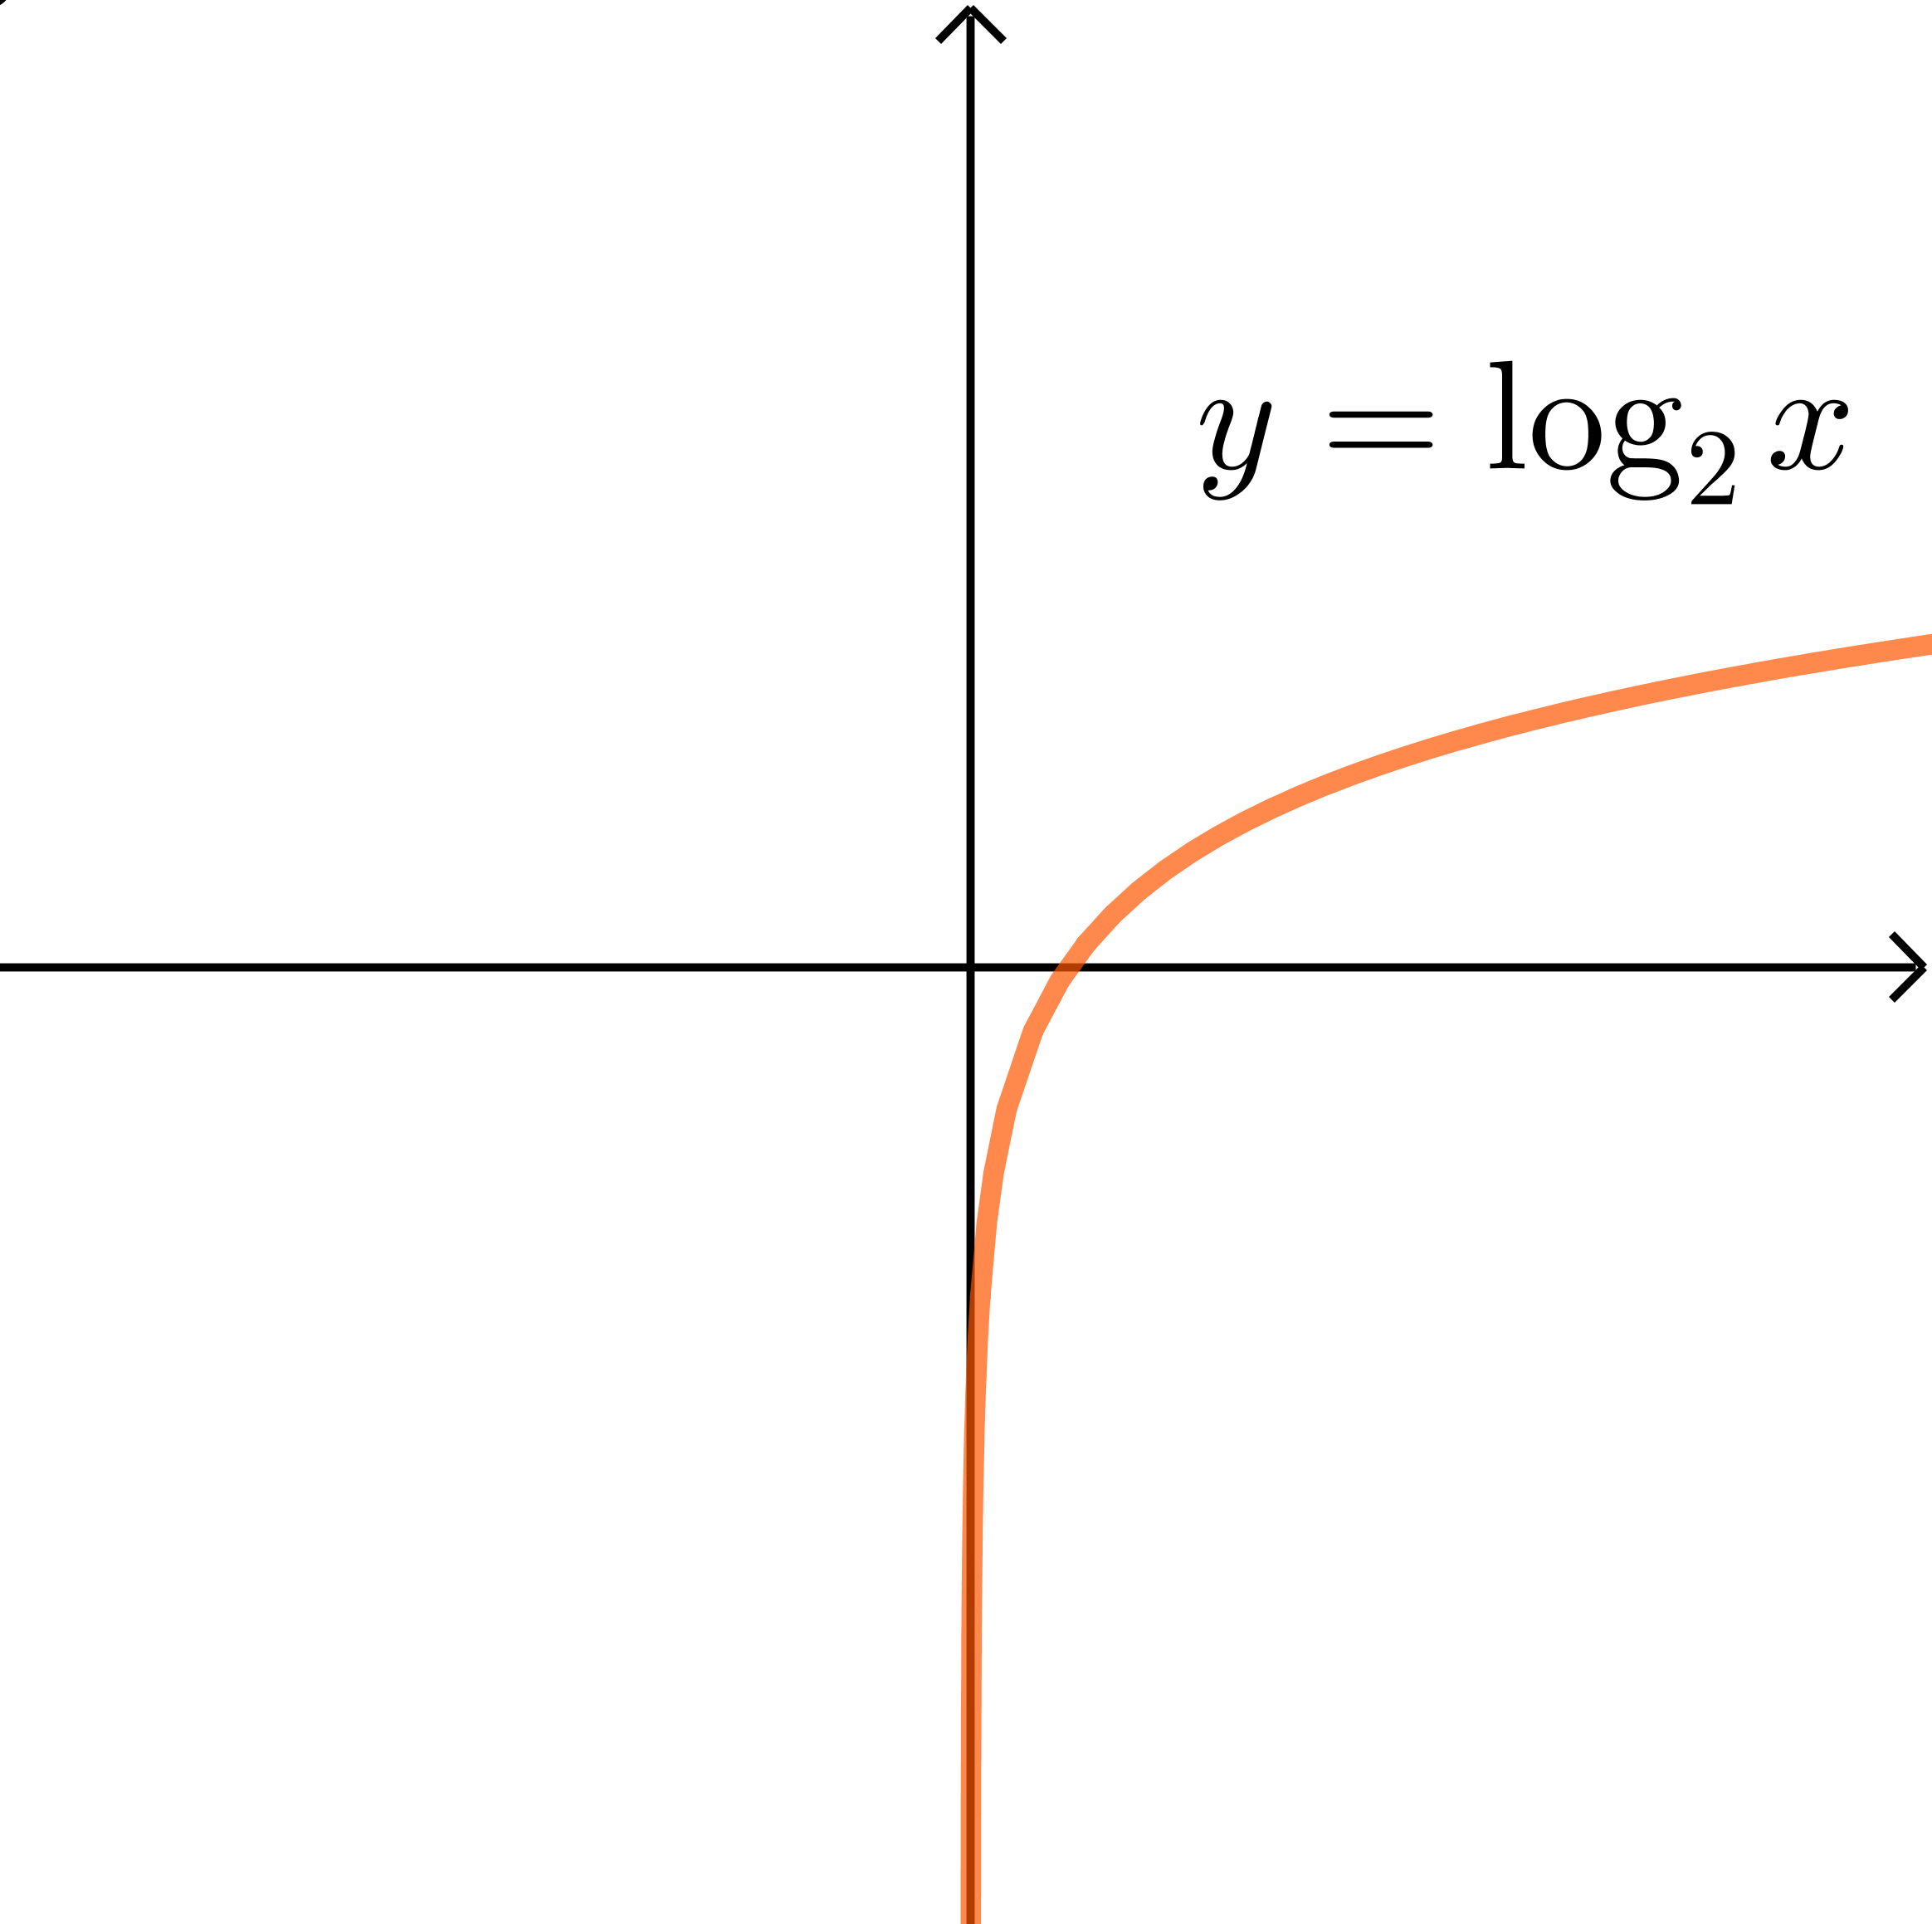
\includegraphics[width=0.3\textwidth]{summary_3}
\qquad\quad
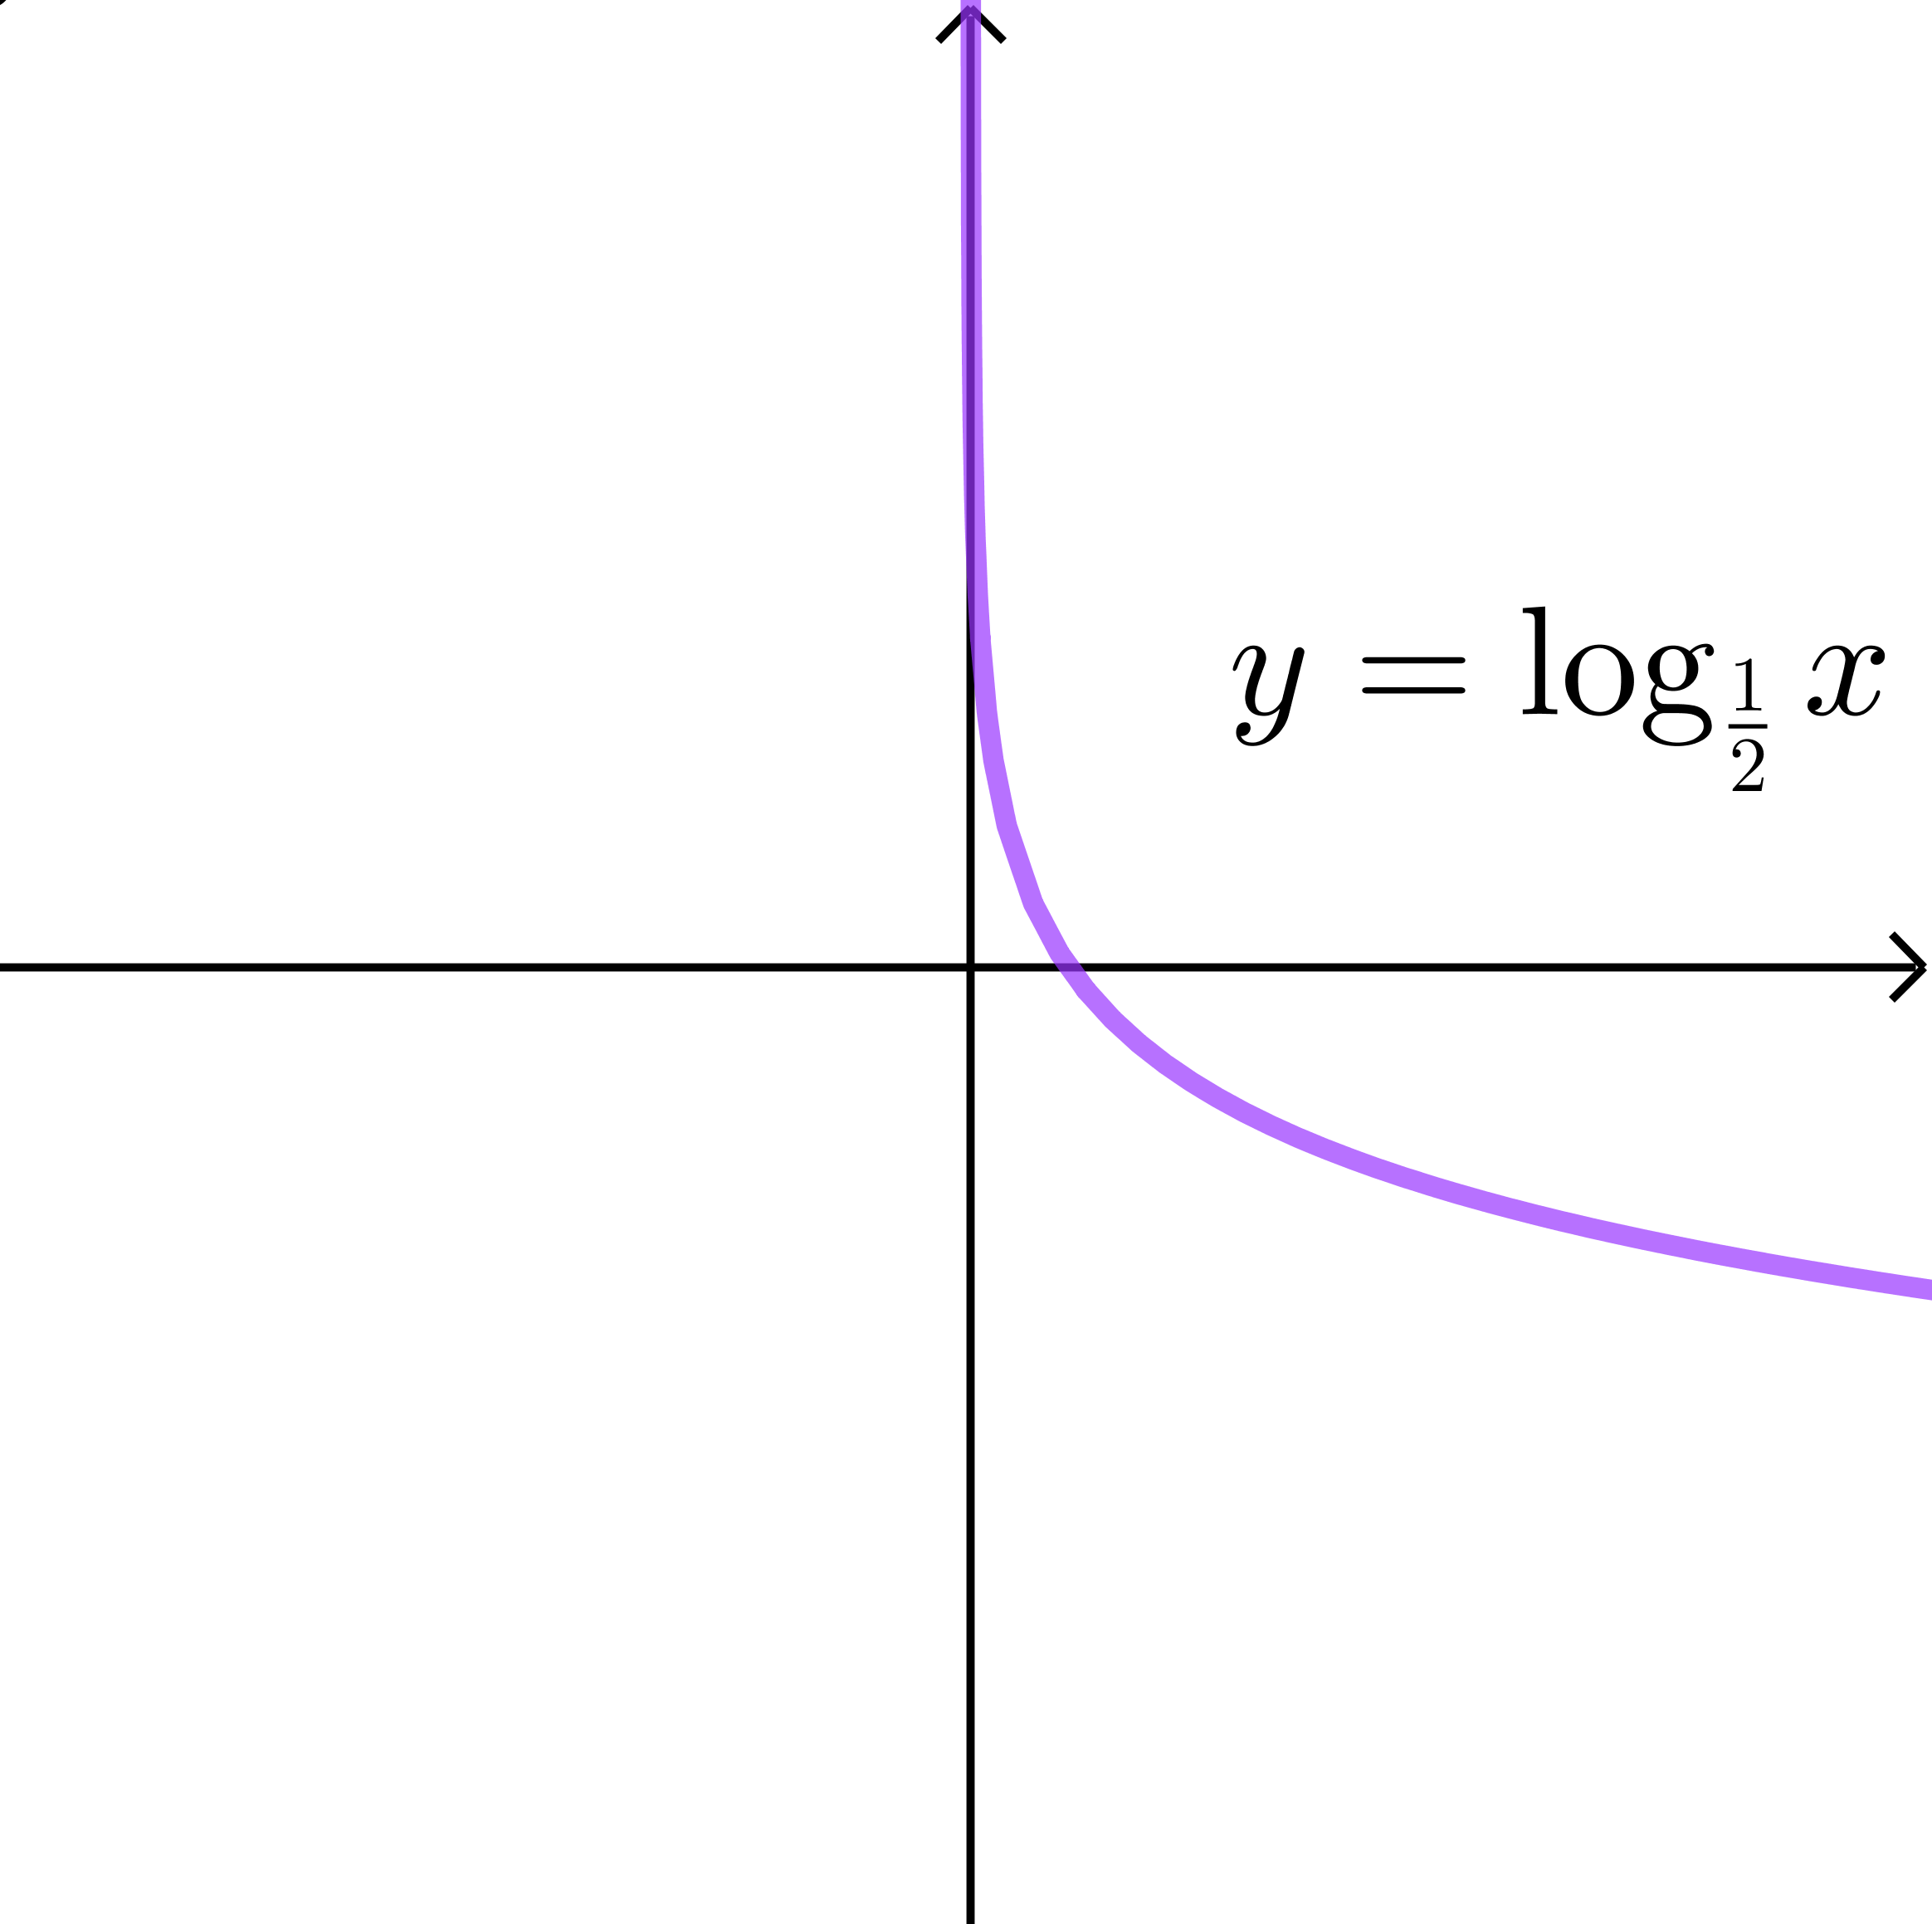
\includegraphics[width=0.3\textwidth]{summary_4}
\end{center}
\item
지수방정식과 로그방정식
\[a^{x_1}=a^{x_2}\quad\Longleftrightarrow\quad x_1=x_2\quad\Longleftrightarrow\quad \log_a{x_1}=\log_a{x_2}\]
\item
지수부등식과 로그부등식
\begin{center}
\(a>1\)일 때,
\(a^{x_1}<a^{x_2}\quad\Longleftrightarrow\quad x_1<x_2\quad\Longleftrightarrow\quad \log_ax_1<\log_ax_2\)\\
\(0<a<1\)일 때,
\(a^{x_1}>a^{x_2}\quad\Longleftrightarrow\quad x_1<x_2\quad\Longleftrightarrow\quad \log_ax_1>\log_ax_2\)
\end{center}

\end{enumerate}
\end{document}